%% 2026-10-15 v8：RQ1快照重算、更新實作與紀錄狀態；RQ2/RQ3仍無正式結果。
%% =====================================================================
%% 多代理人立場交換辯論機制應用於投資決策（初稿）
%% 2026-10-07 v7（最後版：補記憶規則、紀錄完整度表、一律看多檢定、RQ2/RQ3 必要對照、機制指標、放空成本限制）。
%% 2026-10-07 v6（依專題研究標準修訂：限縮結論、釐清 RQ3 定位、補記憶與稽核限制、移除未驗證占位內容，並補直接相關文獻）。
%% 2026-10-07 v5（依邏輯檢查修訂：摘要、動機銜接、模組狀態標示、第五章重排、結論補基準比較）。
%% 2026-10-07 v4（白話版：用字改為大學生程度；字距比照 v2）。v3（依 v2 仔細檢查結果修訂；改用 xelatex + xeCJK 以修正 PDF 文字層）。
%% 2026-10-06 新版研究設計修訂稿（v2：依 SSRN.tex 格式調整編號與版面）。
%% 參考文獻改由 references-meeting-20261006.bib 產生（natbib + chicago，與 SSRN.tex 相同）。
%% 編號：章 1、節 1.1、小節 1.1.1（單一阿拉伯數字層級，不再混用中文數字）。
%% 章節：摘要、引言、文獻探討、研究方法、系統設計與實作、結果與討論、結論與建議、參考文獻
%% =====================================================================

\documentclass[12pt,a4paper]{article}

%% ---------- 套件 ----------
\usepackage{amsmath}
\usepackage{fontspec}
\usepackage{xeCJK}
\setmainfont{Times New Roman}
\setsansfont{Arial}
\setCJKmainfont[Path=C:/Windows/Fonts/,AutoFakeBold=2.5]{kaiu.ttf}
\setCJKsansfont[Path=C:/Windows/Fonts/,AutoFakeBold=2.5]{kaiu.ttf}
%% 字距比照 v2（CJKutf8 + bkai 的疏朗排版）：中文字之間加一點間距
\xeCJKsetup{CJKglue=\hspace{0.1em plus 0.05em minus 0.02em}}
\usepackage[left=3cm,right=3cm,top=3cm,bottom=2cm]{geometry}
\usepackage{graphicx,array,tabularx,booktabs,float}
\usepackage{setspace,enumitem,footmisc}
\usepackage[explicit]{titlesec}
\usepackage{caption}
\usepackage{natbib}
\usepackage{tocloft}
\usepackage{tikz}
\usetikzlibrary{positioning,arrows.meta,calc}
\usepackage[bookmarks=false,hidelinks]{hyperref}

%% ---------- 行距與段落 ----------
\setstretch{1.5}
\setlength{\parindent}{2em}
\setlength{\parskip}{0pt}
\setlist{itemsep=2pt,topsep=4pt,leftmargin=2.5em}
\renewcommand{\arraystretch}{1.6}
\setlength{\tabcolsep}{8pt}
\setlength{\footnotesep}{8pt}
\emergencystretch=2em

%% ---------- 編號：章 第一章；節 第一節；小節 一、 ----------
\newcommand{\chnum}[1]{\ifcase\numexpr#1\relax 〇\or 一\or 二\or 三\or 四\or 五\or 六\or 七\or 八\or 九\or 十\or 十一\or 十二\fi}
\renewcommand{\thesection}{第\chnum{\value{section}}章}
\renewcommand{\thesubsection}{第\chnum{\value{subsection}}節}
\renewcommand{\thesubsubsection}{\chnum{\value{subsubsection}}}
\numberwithin{table}{section}
\numberwithin{figure}{section}
\renewcommand{\thetable}{\arabic{section}-\arabic{table}}
\renewcommand{\thefigure}{\arabic{section}-\arabic{figure}}
\setcounter{tocdepth}{2}
\setlength{\cftsecindent}{0pt}\setlength{\cftsecnumwidth}{4.5em}
\setlength{\cftsubsecindent}{1em}\setlength{\cftsubsecnumwidth}{4em}
\setlength{\cftsubsubsecindent}{5em}\setlength{\cftsubsubsecnumwidth}{2.5em}\renewcommand{\cftsubsubsecaftersnum}{、}
\setlength{\cfttabindent}{0pt}\renewcommand{\cfttabpresnum}{表~}\setlength{\cfttabnumwidth}{4.2em}
\setlength{\cftfigindent}{0pt}\renewcommand{\cftfigpresnum}{圖~}\setlength{\cftfignumwidth}{4.2em}
\renewcommand{\cftsecfont}{\normalfont}\renewcommand{\cftsecpagefont}{\normalfont}
\renewcommand{\cfttoctitlefont}{\hfil\fontsize{16}{24}\selectfont}\renewcommand{\cftaftertoctitle}{\hfil}
\renewcommand{\cftlottitlefont}{\hfil\fontsize{16}{24}\selectfont}\renewcommand{\cftafterlottitle}{\hfil}
\renewcommand{\cftloftitlefont}{\hfil\fontsize{16}{24}\selectfont}\renewcommand{\cftafterloftitle}{\hfil}

%% 小節（一、）的交叉參照：印出「第三章第四節第五項」
\makeatletter
\newcommand{\frlabel}[1]{\protected@write\@auxout{}{\string\global\string\@namedef{fr@#1}{\string\fr@fmt{\number\value{section}}{\number\value{subsection}}{\number\value{subsubsection}}}}}
\def\fr@fmt#1#2#3{第\chnum{#1}章第\chnum{#2}節第\chnum{#3}項}
\newcommand{\frref}[1]{\ifcsname fr@#1\endcsname\csname fr@#1\endcsname\else ??\fi}
\makeatother

%% ---------- 標題 ----------
\titleformat{\section}[block]{\centering\fontsize{18}{27}\selectfont}{\thesection}{1em}{#1}
\titleformat{\subsection}{\fontsize{16}{24}\selectfont}{\thesubsection}{1em}{#1}
\titleformat{\subsubsection}{\fontsize{14}{21}\selectfont}{\thesubsubsection、}{0em}{#1}
\titleformat{\paragraph}[runin]{\fontsize{12}{18}\selectfont}{}{0em}{#1}
\titleformat{name=\section,numberless}[block]{\centering\fontsize{18}{27}\selectfont}{}{0em}{#1}
\titleformat{name=\subsection,numberless}{\fontsize{16}{24}\selectfont}{}{0em}{#1}
\titlespacing*{\section}{0pt}{12pt}{18pt}
\titlespacing*{\subsection}{0pt}{14pt}{8pt}
\titlespacing*{\subsubsection}{0pt}{12pt}{6pt}
\titlespacing*{\paragraph}{2em}{6pt}{0.5em}

%% ---------- 圖表 ----------
\captionsetup{font={small,stretch=1.2},labelsep=space,skip=6pt}
\captionsetup[table]{position=top,justification=raggedright,singlelinecheck=false}
\setlength{\heavyrulewidth}{0.8pt}
\setlength{\lightrulewidth}{0.4pt}
\pagestyle{plain}

\newcommand{\grp}[1]{\textsf{#1}}
\newcolumntype{Y}{>{\raggedright\arraybackslash}X}
\newcolumntype{L}[1]{>{\raggedright\arraybackslash}p{#1\textwidth}}

\begin{document}

\renewcommand{\refname}{參考文獻}
\renewcommand{\contentsname}{目\quad 次}
\renewcommand{\listtablename}{表\quad 次}
\renewcommand{\listfigurename}{圖\quad 次}
\renewcommand{\tablename}{表}
\renewcommand{\figurename}{圖}

%% =====================================================================
%% 封面
%% =====================================================================
\begin{titlepage}
\centering
\setstretch{1.6}
\vspace*{2cm}
{\fontsize{18}{27}\selectfont 國立陽明交通大學管理科學系\par}
\vspace{0.3cm}
{\fontsize{16}{24}\selectfont 專題研究報告\par}
\vspace{3.5cm}
{\fontsize{20}{32}\selectfont 多代理人立場交換辯論機制\\ 應用於投資決策\par}
\vspace{0.3cm}
\vspace{0.5cm}
{\fontsize{14}{21}\selectfont Multi-Agent Role-Switching Debate\\ for Investment Decision-Making\par}
\vfill
{\fontsize{14}{24}\selectfont
\begin{tabular}{r@{\hspace{1.5em}}l}
學\hspace{2em}生： & 黃岳振 \\
指導教授： & 林斯寅\ 教授 \\
\end{tabular}\par}
\vspace{2.5cm}
{\fontsize{14}{21}\selectfont 中華民國一一五年十月\par}
\vspace{1.5cm}
\end{titlepage}

%% =====================================================================
%% 摘要
%% =====================================================================
\pagenumbering{roman}
\begin{center}
{\fontsize{16}{24}\selectfont 摘\quad 要\par}
\end{center}
\vspace{0.3cm}

投資時要同時看股價走勢、公司財報、新聞氣氛和整體經濟狀況，而這些資訊常常互相矛盾。「多代理人辯論」是讓多個 AI 角色分別扮演看多與看空，互相挑毛病，最後由一位裁決者做決定。但只是給 AI 不同的角色，並不代表它們真的會有不同的想法。本研究的核心是「自我反駁式立場交換」：讓 AI 先主張一個立場，再換邊反駁自己，最後回到原本立場整理結論。

本研究規劃三個問題：第一，整套立場交換辯論（D）比起「各守原立場」的整套固定立場辯論（C），有沒有額外的好處；第二，辯論的雙方如果使用不同的 AI 模型，這個好處會不會改變；第三，把四類資訊分給四組專長不同的辯論者處理，結果與成本會不會更好。\textbf{本報告已完成第一個問題；第二、第三個問題目前只完成研究設計，尚未執行，因此本報告不提供它們的結果。}

研究使用九檔美國大型股在 2021 至 2025 年間的 180 個季度案例，每個案例只使用分析日以前已公開的資料，並以資料快照與稽核紀錄控制主要輸入。主要評估指標是 60 個交易日後的方向準確率（猜對漲跌的比例）與年化 Sharpe 比率（每承擔一單位風險能換到多少報酬），另外也看報酬、最大虧損、雙方意見分歧與運算資源。現有版本與原始輸出的保存仍有缺漏，因此本研究將結果定位為指定樣本與流程下的回溯比較，而非可完全重現的確認性檢驗。

第一個問題的 180 案比較結果如下：D 的準確率（55.0\%）與 Sharpe（0.54）沒有比 C（58.3\%、0.59）更高，也就是沒有找到 D 比 C 好的顯著證據。此外，C、D 的準確率都低於「一律看多」的 62.2\%，四組的 Sharpe 也都低於同配置買進持有的 1.01（準確率相對「一律看多」的事後配對檢定也不顯著；Sharpe 相對買進持有則尚未檢定）。要注意的是，D 同時改變了交換立場、隔離對手、強制引用自己原文與驗證重試，所以結果不能歸因於單一的「立場交換」；而且這 180 案先前已用在試跑與規則調整，因此這是規則定好之後對既有樣本的事後回頭比較，不是對全新樣本的確認性檢驗。

\vspace{0.6cm}
\noindent 關鍵詞：大型語言模型、多代理人辯論、立場交換、模型異質性、領域專業化、投資決策

\noindent JEL 分類碼：G11、G17、C53
\clearpage
\begin{center}{\fontsize{16}{24}\selectfont Multi-Agent Role-Switching Debate\\ for Investment Decision-Making\par}\vspace{0.3cm}{\fontsize{14}{21}\selectfont Abstract\par}\end{center}
\noindent Investment decisions require the integration of technical, fundamental, news-sentiment and macroeconomic evidence, which may conflict with one another. Multi-agent debate uses opposing views and adjudication to examine arguments, yet role differences do not necessarily produce useful reasoning diversity. This study centers on self-rebuttal role-switching and plans three research questions: (RQ1) whether the full role-switching debate procedure (D) adds value over the full fixed-role debate procedure (C); (RQ2) whether model composition changes this effect; and (RQ3) whether domain-specialized decision-making improves performance and cost effectiveness. \textbf{This report completes RQ1 only; RQ2 and RQ3 are planned designs that have not been run, and no results are reported for them.}

The study uses 180 quarterly cases of nine U.S. stocks in 2021--2025, integrating four financial information domains under point-in-time data boundaries, immutable snapshots, evidence identifiers and audit trails. The primary evaluation metrics are 60-trading-day directional accuracy and annualized Sharpe ratio, supplemented by return, drawdown, disagreement and inference-resource measures.

For RQ1, D did not outperform C in directional accuracy (55.0\% vs. 58.3\%) or annualized Sharpe ratio (0.54 vs. 0.59), and no significant evidence favoring D was obtained. Point estimates for both C and D also fall below an always-buy benchmark in accuracy (62.2\%) and below a buy-and-hold reference in Sharpe ratio (1.01); a post hoc paired test of accuracy against always-buy was not significant, and the Sharpe comparison was not tested. Because D bundles role-switching, opponent isolation, forced self-quotation and validation retries, the result cannot be attributed to role-switching alone. Because the same sample had been used for pilot work and rule revisions, this is a retrospective comparison under locked rules rather than a confirmatory test.

\vspace{0.6cm}
\noindent Keywords: large language models, multi-agent debate, role switching, model heterogeneity, domain specialization, investment decisions

\noindent JEL Codes: G11, G17, C53
\clearpage
\tableofcontents
\clearpage
\listoftables
\clearpage
\listoffigures
\clearpage
\pagenumbering{arabic}

\clearpage\section{引言}

\subsection{研究背景}

\subsubsection{金融資訊整合與大型語言模型}
做投資決策時，要同時參考股價走勢（技術面）、公司財報（基本面）、新聞氣氛（情緒面）和整體經濟狀況（總體經濟面）。這些資訊更新的速度、呈現的形式，甚至指向的方向都可能不一樣。大型語言模型（例如 ChatGPT 這類 AI）可以幫忙閱讀財報、新聞和市場資料，已有不少研究把它用在金融文字分析與投資分析 \citep{lopezlira2023chatgpt,araci2019finbert,liu2023fingpt}。不過，「把資訊整理好」和「預測未來報酬」是兩件不同的事；AI 的說明寫得有條有理，不代表它真的能預測股價。

\subsubsection{多代理人辯論與立場交換}
多代理人辯論，是讓多個 AI 角色輪流提出論點、批評對方、修正自己 \citep{du2023debate,liang2023divergent}。金融領域的 AI 系統也常把工作分成分析與交易等角色 \citep{xiao2024tradingagents,zhang2024stockagent}。但辯論好不好用，要看用什麼模型、怎麼互動、怎麼裁決，並不一定比單一模型或「多問幾次再投票」更好 \citep{smit2023mad,zhang2025stop}。因此，辯論流程怎麼設計，本身就是值得研究的問題。

本研究主要比較兩種辯論方式。C 組是「固定立場辯論」：看多方一直站在看多，看空方一直站在看空。D 組是「自我反駁式立場交換」：第二輪時，每個角色只看自己第一輪寫的內容，然後換到相反立場，引用並反駁自己原本的主張；第三輪再回到原本立場，把剛剛找到的反面證據整理進結論。本研究想了解，這種「逼自己重新檢查證據」的做法，有沒有額外的價值，並進一步看它會不會受到模型組合與資訊分工方式的影響。

\subsection{研究動機}

\subsubsection{自我反駁機制有沒有額外價值}
多代理人辯論到底有沒有用，目前仍有爭議。有些研究發現辯論能提高推理的正確率 \citep{du2023debate}，但也有研究發現辯論不一定比「同一個問題問多次再投票」好，而且辯論的效果常被高估 \citep{smit2023mad,zhang2025stop}。辯論有一個常見的問題：角色會「死守立場」，只會加強自己的論點，不回應對方的證據。立場交換就是為了緩和這個問題而提出的 \citep{liu2025roleswitch,chowdhury2026proclaim}。這些研究讓我們有理由期待立場交換可能有用，但它們處理的是問答或事實查核，和預測未來股價報酬不同。所以本研究直接拿 C、D 兩種流程，在相同資料、相同預定決策呼叫次數下比較。

另外，股票回測很容易失真。AI 模型可能在訓練時就已經看過回測期間之後的股價走勢，等於「偷看答案」\citep{glasserman2023lookahead,kong2026bias}；辯論組通常也比單次判斷多用好幾倍的模型呼叫次數。因此，本專題希望在控制這些問題的前提下，檢驗立場交換在投資情境裡是否真的有用。

RQ1 的結果（見第五章）沒有找到 D 優於 C 的證據。文獻與系統設計上，有兩個條件可能限制這類機制的效果：辯論雙方由同一個模型擔任，以及四類資訊合併處理。以下兩項是\textbf{候選假說}，本研究並沒有證明它們就是 RQ1 結果的原因；RQ2 與 RQ3 的目的，是在受控條件下檢驗這兩個條件是否真的改變結果。

\subsubsection{同一個模型扮演雙方，想法可能不夠多元}
看多（Bull）與看空（Bear）兩個角色雖然被要求主張相反的立場，但如果背後是同一個 AI 模型，它們可能有相同的知識盲點、相同的推理習慣，也會犯相同的錯。角色不同，不保證想法真的不同；改用不同的模型是否能互相補足，還需要檢驗 \citep{zhang2025stop}。另一方面，不同模型的能力、訓練資料與寫作風格本來就不一樣，所以換了模型之後績效出現差異，不能直接說是「模型不同」造成的。

\subsubsection{通才組把資訊集中處理，專才組分工處理}
目前系統已有四個研究代理人，負責整理四類資訊，但真正做判斷的仍只有同一組看多與看空。技術、基本、新聞情緒與總體經濟這四類證據，更新速度和訊號性質各不相同；全部合在一起處理，可能讓某一類資訊的反面證據被稀釋，也可能讓模型一次要讀的內容太多。這是候選假說，並非已被 RQ1 的結果證實的原因。RQ3 打算讓四類資訊各自有自己的多空辯論，再由上層整合，然後評估這樣做的好處、意見衝突與額外成本。

\subsection{研究目的}

\subsubsection{立場交換機制}
檢驗「自我反駁式立場交換」相較於固定立場辯論，有沒有額外的價值。這是本研究最原始的核心問題。

\subsubsection{模型異質性}
檢驗辯論雙方使用的模型組合，會不會改變 D 相對於 C 的效果，並分辨「角色不同」與「模型不同」各自的影響。

\subsubsection{領域專業化}
檢驗「領域內辯論加上上層整合」相對於通才（Generalist）做法的績效與成本，評估把任務拆分是否划算。

\subsection{研究問題}

\subsubsection{RQ1：原始機制}
\begin{quote}在相同的案例資料與相同的預定決策呼叫次數下，自我反駁式立場交換辯論（D）的 60 日方向準確率與年化 Sharpe，是否高於固定立場辯論（C）？\end{quote}

\subsubsection{RQ2：模型異質性}
\begin{quote}當看多與看空代理人由不同的基礎模型擔任時，自我反駁式立場交換辯論（D）相對於固定立場辯論（C）的投資決策效果，是否會改變？\end{quote}

\subsubsection{RQ3：領域專業化辯論}
\begin{quote}原本是把四類金融資訊合併後，交給同一組多空代理人辯論。若改為讓技術面、基本面、情緒面與總經面代理人，各自在自己的資訊範圍內進行多空辯論，再由上層整合機制做出最終決策，方向準確率與風險調整後績效是否會更好？\end{quote}
RQ1 與 RQ2 構成主要研究線：先比較整套 C、D 流程，再檢驗模型組合是否改變兩者差異。RQ3 則是平行的系統架構延伸，檢驗資訊分工與額外運算成本的整體取捨；它不直接檢驗立場交換本身，而且比較的是「整套領域化架構」，結論不稱為單純的分工效果。

\subsection{研究範圍}

\subsubsection{樣本與資料時間邊界}
本專題是投資決策輔助的研究與系統原型，不是會自動下單的交易系統。研究範圍整理於表~\ref{tab:scope}。

\begin{table}[H]
\centering\small
\caption{研究範圍}
\label{tab:scope}
\begin{tabularx}{\textwidth}{@{}l Y@{}}
\toprule
項目 & 說明 \\
\midrule
標的與期間 & 九檔美國大型股；2021 至 2025 年每季取一個分析日，共 180 個案例 \\
資料 & 技術面、基本面、情緒面（新聞標題）與總經面；只使用分析日以前已經公開的資料 \\
決策輸出 & 買進、持有或賣出，並附上預期報酬、信心度、理由、引用的證據與風險 \\
評估 & 60 個交易日後的方向準確率與 Sharpe 比率；30 與 90 日用來檢查結果穩不穩 \\
\bottomrule
\end{tabularx}
\end{table}
\subsubsection{預測期間與決策層}

本研究維持九檔股票、20 個季末、共 180 個「股票 $\times$ 日期」案例，預測期間為 60 個交易日。C、D 兩組的候選決策只能在買進與賣出之間選一個；之後的「守門員」（Gatekeeper）可以把決策降為持有或不交易。A、B 兩組允許選持有，只作為補充對照。主要分析使用守門員之前的候選決策；經守門員處理後的實際結果，另外作為敏感性分析。以月（約 20 個交易日）為單位的比較屬於未來研究，本研究的季度樣本不變。

\subsubsection{研究狀態與證據界線}
各部分目前的進度整理於表~\ref{tab:status}。已經做完的，是在既有「季度實驗規則」下的事後回頭比較（回溯比較）。RQ2、RQ3 與月度設計都還只是設計，設計中預期的好處不能當成已有的結果。

\begin{table}[H]
\centering\small
\caption{研究狀態}
\label{tab:status}
\begin{tabularx}{\textwidth}{@{}L{.30} L{.17} Y@{}}
\toprule
項目 & 狀態 & 能說明到什麼程度 \\
\midrule
RQ1：D 對 C（qwen3:32b，季度實驗規則 v3-1002.3） & 已完成 180 案 & 這是規則定好後對既有樣本的事後比較。沒有找到 D 優於 C 的顯著證據，但這不等於兩者一樣好 \\
Gemini 3 Flash 同批比較 & 已報告（探索性） & 整套系統換成同一個別的模型，不是 RQ2；用的還是同一批案例，不算獨立重做 \\
RQ2：模型組成 & 設計階段，未執行 & 比較方式與配置規則見\frref{sec:rq2design}；尚無結果 \\
RQ3：領域分工 & 設計階段，未執行 & 流程與資源比較見\frref{sec:rq3design}；尚無結果 \\
月度／20 日設定 & 未執行 & 另外獨立設計，不併入這 180 個季度案例 \\
\bottomrule
\end{tabularx}
\end{table}

\clearpage\section{文獻探討}

\subsection{多代理人辯論}

\subsubsection{辯論與「多次取樣投票」的公平比較}
\citet{du2023debate} 讓多個模型實例進行多輪辯論後收斂出答案，使推理與事實正確性變好。\citet{liang2023divergent} 指出模型自我反省時容易死守原本的答案，因此用辯論來鼓勵多元思考。但另一方面，\citet{smit2023mad} 比較了多種辯論策略，發現多代理人辯論不一定比「自我一致性」等其他方法穩定地好，而且對設定很敏感；\citet{zhang2025stop} 則認為目前的評估常高估辯論的效果，建議重新思考評估方式，並改用不同的模型。「自我一致性」\citep{wang2023selfconsistency} 是指同一個問題問多次、再用多數決選答案。這能讓結果更穩定，也是比較辯論效果時必要的對照組；本研究的「獨立投票組」（B 組）就是依此設計。因此，本研究把重點放在流程可追蹤、比較公平（模型呼叫次數對齊），而不是先假設辯論一定比較準。
\subsection{角色交換與自我反駁}

\subsubsection{為什麼可能有效，又為什麼可能無效}
\citet{liu2025roleswitch} 提出「會考慮不確定性的角色交換辯論」：兩位辯論者先各自給出初步答案並互相質問，辯論到一半時交換角色、改為論證相反立場，然後各自回報信心與不確定性，最後由另一個裁判模型決定。在 OpenBookQA（問答題庫）上，他們的消融實驗（把某個步驟拿掉看結果變化）顯示，角色交換與回報不確定性兩個階段都有貢獻。\citet{chowdhury2026proclaim} 的 PROCLAIM 以法庭角色（原告、辯護、法官）搭配逐步檢索來查核主張，並用角色交換檢查答案是否一致；其消融結果顯示角色交換約使準確率提高 4.2 個百分點，但整體 token 用量約為標準多代理人辯論的 11 倍。\citet{chen2026mpt} 的多人格思考則讓相反的人格與中立觀點反覆對話，使偏誤被說出來並被修正。這些研究支持「從相反立場重新想一次」這個想法，但它們都不是投資決策，而且其中 PROCLAIM 的好處是靠大幅增加成本換來的，這也說明為什麼比較時必須讓模型呼叫次數相同。本研究因此採用「看多、看空、裁決者」三方架構，並讓獨立投票組與兩個辯論組的決策呼叫次數對齊（單次判斷組為基準）。\paragraph{機制的動機與可能失效的情況。}
\citet{lord1984opposite} 的人類社會判斷實驗指出，主動考慮「與自己原本信念相反的可能性」，可以減少特定的判斷偏誤。本研究據此提出假說：要求 AI 引用並反駁自己的論點，也許能挖出先前被忽略的反面證據，讓裁決者更平衡地衡量證據。不過，這個推論是從人類實驗延伸到 AI 預測股價，仍需實際檢驗；論述寫得更完整，也不一定代表預測得更準。\citet{huang2024selfcorrect} 發現，沒有外部回饋的自我修正，在其測試的推理題上可能沒效果，甚至讓表現變差。如果模型共享相同的錯誤、輸入資訊本身缺乏預測力，或市場雜訊太大，自我反駁也可能只是改變說法，績效並沒有進步。


\subsection{多代理人系統中的模型異質性}

\subsubsection{模型不同、能力不同與模型偏好}

\citet{zhang2025stop} 檢驗了多代理人辯論的評估方式與模型異質性（用不同的底層模型），讓我們有理由研究不同模型一起推理的效果。但他們的基準測試結果，不能直接套用到金融未來報酬預測，也不能直接套用到本研究的自我反駁規則。RQ2 要做的，是在同一場辯論裡同時放進 M1、M2 兩種模型；這和「整套系統都換成另一個模型」不同，後者仍然是單一模型的做法（homogeneous setting）。模型的能力高低、偏好、裁決者對某種文風的偏愛，以及不同模型犯錯的相關性，都必須分開檢查。

\citet{wang2024moa} 的 Mixture-of-Agents 把多個模型的輸出一層一層地整合，並比較「同一模型重複生成」與「多個模型各自提案」的差別。該研究也把「提出方案」與「整合方案」分成不同角色，顯示同一個模型放在流程的不同位置，適用程度可能不同。本研究據此把模型組合當成實驗要操弄的因素，並固定裁決者；不過，該研究是一般語言任務，結果不等於不同模型的金融辯論就有效，也不能排除只是模型能力有差距。

\subsection{金融領域的語言模型與投資代理人}

\subsubsection{金融文字分析與代理人流程}
\citet{lopezlira2023chatgpt} 在其樣本與設定中發現，大型語言模型對金融新聞標題的判讀，含有與後續報酬相關的訊息。FinBERT \citep{araci2019finbert} 與 FinGPT \citep{liu2023fingpt} 提供了金融文字處理的方法，FNSPID \citep{dong2024fnspid} 則提供有時間戳記的新聞資料。這些研究說明了資訊整理可能有用，但並不能直接證明任何一種辯論流程有額外價值。

TradingAgents \citep{xiao2024tradingagents} 與 StockAgent \citep{zhang2024stockagent} 把 AI 分工與交易決策放在回測或模擬環境中檢驗；它們的研究對象是整套代理人系統，和本研究「先固定案例輸入，再比較 \grp{D}、\grp{C}」的做法不同。\citet{glasserman2023lookahead} 對「偷看未來」風險的分析，以及 \citet{huang2024selfcorrect} 對「沒有外部回饋的自我修正」的謹慎結果，都提醒研究者：推理流暢、模擬績效漂亮，並不能單獨證明模型有可用的預測能力。因此，本研究把缺口限定為：在預定決策呼叫次數相同、資料時間邊界可以被查核的條件下，檢查「重新審視既有證據」的自我反駁流程，能不能改善方向準確率與風險調整後績效；而不是單純把現成的辯論方法搬到金融領域。

近期也已有研究直接檢查多代理人辯論的論證品質與金融績效關係。\citet{huang2026explainabletrading} 在歷史市場模擬中發現，較高的整體論證品質未必伴隨較高的 Sharpe 或總報酬，顯示「論證看起來更好」與「經濟結果更好」必須分開評估。該研究著重投資組合配置、論證品質與分歧維持；本研究則比較固定立場與自我反駁式立場交換的整套流程，兩者的研究對象不同，但都支持以金融績效而非文字品質作為主要判準。
\subsection{領域專業化與任務拆分}

\subsubsection{「整理資料」分工與「做決策」分工的差別}
TradingAgents 與 StockAgent 提供了金融代理人工作流程的背景 \citep{xiao2024tradingagents,zhang2024stockagent}。FinRobot 把金融任務拆給不同的專業代理人，並用分層流程處理，是金融問題拆解與工具串接的一個例子 \citep{yang2024finrobot}；但它並沒有提供本研究「四領域多空辯論 vs. 通才架構」的受控績效比較。

\citet{chen2023agentverse} 的 AgentVerse 把流程分成專家配置、協作決策、執行與評估，並討論水平與垂直兩種協作結構，說明代理人怎麼分工、怎麼溝通，會共同影響決策的過程。因此，RQ3 把專業化從「資料整理層」延伸到「領域內推理」與「上層整合」。要說明的是，把資訊切成四個領域，是本研究自己的設計選擇，並不是既有研究證明過的最佳架構。

把資訊按領域切開，可能保留每個領域的反面證據，但也可能遺失跨領域的關聯、增加摘要時壓縮資訊的損失，並帶來整合時的誤差。與其只用「模型一次讀不下太多內容」來解釋分工，本研究更關心：專業化要不要進到「決策推理」這一層？並用績效、證據使用與推論資源，來評估其中的得失。

\subsection{裁決、整合與驗證}
\subsubsection{產生論證、上層整合與證據驗證}
Mixture-of-Agents 把「提出方案」與「上層整合」分開 \citep{wang2024moa}，提供了不同角色分別負責論證與整合的架構參考。\citet{zheng2023judge} 指出，用大型語言模型當裁判時，可能出現偏好排在前面的答案、偏好較長的答案、偏好自己產生的答案等偏誤，所以裁決時輸入的順序、長度與模型標籤都需要控制。不過，該研究評估的是「回答品質」，並不能直接證明本研究的投資裁決者有預測能力。

本研究據此把「產生論證」、「整合決策」與「驗證證據」分成三個可以被查核的步驟。裁決者（Judge）或最終整合者（Final Aggregator）綜合各方論點，決定方向；守門員（Gatekeeper）則檢查證據是否真的存在、資料是否足夠，以及風險是否過高。守門員是本系統自己的驗證設計，本研究不以一般的 AI 裁判文獻，來說明它能改善投資績效。

\subsection{偷看未來的問題與金融評估}

\subsubsection{資料時間邊界與模型的訓練記憶}
\citet{glasserman2023lookahead} 指出，用 GPT 產生情緒訊號去預測報酬時，模型可能因為本來就知道這些公司的後續發展，而產生「偷看未來」的偏誤（前視偏差），並嘗試用匿名化來緩和。\citet{kong2026bias} 整理出金融語言模型研究中常見的五種偏誤（前視、存活、敘事、目標與成本偏誤），並指出多數研究沒有明確處理這些問題。因此，本研究在資料端嚴格排除分析日之後的資訊，並用前導階段做的「資料回想」與「匿名辨識」兩項探針，作為初步的風險檢查（見\frref{sec:memorydiagnostic}），回測時也扣除交易成本。不過這些探針並不是新版主樣本完整的汙染檢驗。
\subsection{文獻小結與研究缺口}

\subsubsection{從機制、模型到任務分工的連續問題}

本研究承接辯論、自我一致性、角色交換、金融文字處理與前視偏差等文獻，先從最基本的問題開始：資料固定時，自我反駁是否有額外價值？再往下檢驗，指定的模型組合與領域分工，是否會改變決策。現有文獻還不足以證明，是「模型太相似」或「資訊太多」才使 RQ1 沒看到績效進步；RQ2 與 RQ3 檢驗的正是這兩個候選假說。三個研究問題提供的是可被查核的比較，而不預設哪種架構一定比較好。此外，文獻中的問答正確率、事實查核與投資報酬預測，評估的目標並不相同，不能直接畫上等號。

\clearpage\section{研究方法}

\subsection{研究架構}

\subsubsection{共用資料層與三個實驗分支}

系統原有的協調者（Coordinator）、資料快照（Data Snapshot）與四類研究代理人（Research Agents）都保留。共用資料層會產生一份「不帶投資方向」的鎖定研究資料與證據登錄。RQ1、RQ2 讀的是同一份中立報告（Neutral Report）；RQ3 的通才組也讀這份整合報告，而領域組則使用同一份研究輸出依領域切開的部分，不另外抓新資料，也不用別的摘要模型重做輸入。整體概念架構如圖~\ref{fig:flow}。
\begin{figure}[H]
\centering
\begin{tikzpicture}[font=\footnotesize,>={Stealth[length=2mm]},
  box/.style={draw=black!55,rounded corners=3pt,align=center,inner sep=4pt,minimum height=8mm,fill=white},
  shared/.style={box,fill=blue!6,draw=blue!50!black,text width=13.4cm},
  done/.style={box,draw=teal!60!black,fill=teal!12,thick,text width=4.3cm,minimum height=21mm},
  plan/.style={box,draw=orange!75!black,fill=orange!8,thick,dashed,text width=4.3cm,minimum height=21mm},
  post/.style={box,draw=black!60,fill=black!4,text width=13.4cm},
  arr/.style={->,thick,black!65}]
% 共用資料層底框
\draw[rounded corners=5pt,draw=blue!40,fill=blue!3,dashed] (0.1,0.8) rectangle (14.9,-2.6);
\node[anchor=south west,font=\scriptsize\sffamily,text=blue!50!black] at (0.1,0.85) {共用資料層（三個分支讀同一份）};
\node[shared] (data) at (7.5,0) {資料來源：行情、財報、新聞標題、總經\\依申報日、歷史版本與時間戳記篩選};
\node[shared] (snap) at (7.5,-1.7) {不可變資料快照 $\rightarrow$ 四個研究代理人 $\rightarrow$ 中立報告與證據登錄};
\draw[arr] (data) -- (snap);
% 三個分支
\node[done] (rq1) at (2.5,-4.9) {\textbf{RQ1}（已完成）\\同一模型 M1/M1\\\grp{C} 對 \grp{D}\\讀同一份中立報告};
\node[plan] (rq2) at (7.5,-4.9) {\textbf{RQ2}（設計階段）\\不同模型 M1/M2\\\grp{C} 對 \grp{D}\\配置 X、Y 平衡};
\node[plan] (rq3) at (12.5,-4.9) {\textbf{RQ3}（設計階段）\\通才組 對 領域專業化組\\四領域各自多空辯論\\（規則 \grp{C}）};
\foreach \n in {rq1,rq2,rq3}{\draw[arr] (\n.north |- snap.south) -- (\n.north);}
% 裁決層
\node[box,text width=9.3cm,minimum height=11mm] (judge) at (5,-7.3) {裁決者（固定；逐項核對證據後擇一方向）};
\node[box,text width=4.3cm,minimum height=11mm] (agg) at (12.5,-7.3) {最終整合者\\（RQ3；本身即最上層裁決）};
\draw[arr] (rq1.south) -- (rq1.south |- judge.north);
\draw[arr] (rq2.south) -- (rq2.south |- judge.north);
\draw[arr] (rq3.south) -- (agg.north);
% 守門員與回測
\node[post] (gate) at (7.5,-9.0) {守門員：檢查證據引用、資料覆蓋、波動度與風險；必要時降級};
\draw[arr] (judge.south) -- (judge.south |- gate.north);
\draw[arr] (agg.south) -- (agg.south |- gate.north);
\node[post] (back) at (7.5,-10.5) {回測 $\rightarrow$ 準確率／Sharpe／成本／診斷};
\draw[arr] (gate) -- (back);
% 圖例
\node[draw=teal!60!black,fill=teal!12,thick,rounded corners=2pt,minimum width=9mm,minimum height=4mm] (l1) at (3.8,-11.6) {};
\node[anchor=west,font=\scriptsize] at (l1.east) {實線：已完成};
\node[draw=orange!75!black,fill=orange!8,thick,dashed,rounded corners=2pt,minimum width=9mm,minimum height=4mm] (l2) at (8.3,-11.6) {};
\node[anchor=west,font=\scriptsize] at (l2.east) {虛線：設計階段，尚未執行};
\end{tikzpicture}
\caption{研究概念架構。三個分支共用同樣的資料、候選決策與評估方式；實線為已完成，虛線為設計階段（尚未執行）。}
\label{fig:flow}
\end{figure}

\subsubsection{裁決者與守門員}

裁決者（Judge）綜合辯論內容、核對證據，並決定投資方向。最終整合者（Final Aggregator）只用在 RQ3，負責整合四個領域的看法；它本身就是最上層的裁決者，因此不再另外設一位決策裁決者。守門員（Gatekeeper）在投資方向決定之後才出場，檢查證據引用、資料覆蓋、波動度、風險門檻與基準率歷史，必要時把決策降級；它不負責整合四個領域的投資觀點。

\subsection{資料收集}

\subsubsection{四類資料與時間控制}
樣本是九檔美國大型股（AAPL、\allowbreak NVDA、\allowbreak GOOGL、\allowbreak MSFT、\allowbreak AMZN、\allowbreak JPM、\allowbreak MCD、\allowbreak INTC、\allowbreak GE），分析日為 2021 至 2025 年共 20 個季末。每個案例只用分析日以前就已公開的資料（表~\ref{tab:data}）：財報依「申報日」而不是「會計期末」篩選；總經資料使用當時實際已發布的歷史版本；資料快照以內容的「雜湊值」（可想成這份資料的指紋碼，內容一改就會不同）來辨識，四組決策機制讀的是同一份快照。

\begin{table}[H]
\centering\small
\caption{資料來源與處理方式}
\label{tab:data}
\begin{tabularx}{\textwidth}{@{}L{.10} L{.25} Y@{}}
\toprule
類別 & 來源 & 內容與處理 \\
\midrule
技術面 & 調整後日行情 & 近 20 日報酬、均線相對位置、年化波動度；只用分析日以前的價格 \\
基本面 & SEC 財報 & 營收、淨利、營業現金流，並與去年同期比較；依申報日篩選 \\
情緒面 & 金融新聞標題（FNSPID、Alpha Vantage） & 分析日前 90 天的全部標題（既有資料共 83,093 則），以 FinBERT 逐則評分後彙整 \\
總經面 & FRED／ALFRED & 失業率、利率、物價等，只採分析日當時已發布的數值 \\
\bottomrule
\end{tabularx}
\end{table}

九檔股票主要依「資料取不取得到」挑選，不是從 2021 年的成分股中隨機抽出。實驗規則記錄了兩項調整：新聞來源沒有涵蓋的 ASTS 被排除；早期新聞有缺口的 LLY 被換成 INTC。所以樣本是有目的地挑選的，也有存活偏誤的風險（只看到活下來的公司）。主要比較保留全部 180 案；先前排除 37 案的分析，只當成新聞來源與覆蓋範圍的診斷，不用它的結果去訂一個統一的新聞數量門檻。

\subsubsection{資料品質與版本風險}
為了讓快照只反映分析日當時能知道的資訊，本研究做了三件事。第一，財報依申報日期而不是會計期末篩選，並且用相同會計科目、相同期間長度與去年同期比較，避免把不同期間混在一起。第二，年增率的分母用前期的絕對值，這樣當基期是負數、狀況又變差時，年增率會是負的，不會因為正負號而誤導。第三，快照以雜湊值識別，同一個模型、同一個案例的四組決策機制，讀的都是同一份快照與鎖定報告。行情使用 yfinance 的 auto\_adjust=True；調整係數反映的是「下載當下」的拆股與股利處理，並不是各分析日當時保存的版本，因此仍有事後被修訂的風險。

在時間上，新聞依發布時間與時區篩選，財報以申報日判斷「何時才看得到」，總經資料用分析日當時已發布的歷史版本，價格輸入只使用截止時間以前的資料。每個案例都會記錄資料版本、快照雜湊值、證據編號、程式版本、模型版本與稽核紀錄。不過，「各組共用同一份快照」並不能單獨證明資料內容是對的，還必須檢查資料的可用時間與來源。模型版本、新聞來源與行情調整版本，都會影響能不能精確重現結果，所以要和快照、執行紀錄一起保存。

\subsection{研究設計選擇與理由}
\begin{table}[H]\centering\small
\caption{主要設計選擇及其用途}
\begin{tabularx}{\textwidth}{@{}L{.17} L{.19} Y@{}}\toprule
設計 & 設定 & 理由 \\\midrule
辯論者 & 看多與看空 & 用兩個相反的方向，建立最簡單的多空論證結構。\\
辯論輪次 & 三輪 & D 組：第一輪提出論證、第二輪自我反駁、第三輪整合修正。C 組：三輪都維持原立場，並依看得到的內容批評與整合。輪數只是操作上的選擇，不宣稱是最佳的。\\
交換時點 & 第二輪 & 先有可以引用的原始主張，再要求從反方向檢查。\\
交換輪能看到的資訊 & 只有自己的第一輪 & 把反駁的對象限定為自己的主張，避免變成模仿對手。\\
第三輪 & 回到原立場 & 把反面證據與不確定性整合進來，觀察修正後的論點。\\
裁決與驗證 & 裁決者之後接守門員 & 把「決定方向」、「證據是否有效」與「風險控制」分成三件事。\\
主要比較 & C／D 預定呼叫次數相同 & 控制其中一項推論資源的差異；實際用掉的 token 與重試成本另外報告。\\
分析頻率 & 每季一次 & 配合財報按季更新的節奏，並沿用既有資料流程與 20 個決策時間點。\\
主要期間 & 60 個交易日 & 當作季度研究的實際持有期間；30 與 90 日用來檢查結果對期間敏不敏感，不宣稱 60 日在理論上最好。\\
資訊領域 & 技術、基本、情緒、總經 & 沿用既有四類證據，區分「整理資料」與「做決策」兩層的專業化。\\\bottomrule
\end{tabularx}\end{table}
各組共通的輸出格式與一般性的證據驗證設定，屬於實作上的參數，與 C／D、模型組合、任務架構等「研究要比較的因素」分開記錄。D 組專屬的「自我引用驗證」，以及驗證不過時觸發的重試，則是整套 D 流程的一部分，和立場交換、資訊隔離一起構成要比較的對象。

\subsection{實驗設計}

\subsubsection{共同的實驗設定}
各條件使用相同的案例、資料快照、結果（outcome）與回測。研究代理人用的模型與輸出、中立報告與證據登錄都固定，避免更換辯論者時，同時改變了輸入資訊。C、D 兩組的三輪辯論與裁決者呼叫次數對齊；模型設定、提示詞指紋碼、實際的隨機種子、token 用量與重試次數，都記錄在稽核紀錄中。

「記憶」只包含分析日以前已經「到期」（60 日結果已經揭曉）的同一檔股票案例，禁止讀取該案例本身的未來報酬，也禁止讀取其他條件的測試結果。RQ1 目前的設定是：C、D 的裁決者可以讀這類已到期記憶，A、B 不行（見\frref{sec:memory}）。依研究服務程式讀取記憶的規則，系統只取「相同實驗規則雜湊值、同一檔股票、同一組別、相同期間與成本模型」的過去案例，且該案例的到期日與分析日都必須早於目前案例的分析日，只取經守門員處理後的決策、排除降級案例，每組最多取最近 20 筆。也就是說，C 與 D 各自只讀自己這一組過去的決策與對錯，彼此隔離，不會讀到另一組的決策；D 的記憶內容是 D 自己過去決策的結果，和 C 不同，這也是「整套流程」差異的一部分。

須注意的是，以上記憶的時間與條件邊界已於 2026 年 10 月 15 日由封存快照核對，但其語意影響與原執行環境的完整重現仍有限制（見\frref{sec:repro}）；在核對完成前，本文不把 C、D 的差異解讀為單一機制的因果效果。RQ2、RQ3 若執行，必須讓各條件的記憶彼此隔離：每個條件只讀自己已到期的案例，不共享決策，並逐案記錄當時可讀內容與到期規則。由於後面案例的輸入會受到前面決策的影響，比較的是「整套流程動態運作的效果」，而不是各次獨立判斷的差異。模型服務的版本與內容被截斷的情形，也必須記錄。

\subsubsection{四組決策機制}
A 組（單次判斷）與 B 組（七次獨立投票）只當作補充對照，主要比較是 C 與 D。四組的流程如表~\ref{tab:arms}。\grp{B}、\grp{C}、\grp{D} 三組的決策呼叫次數對齊（各 7 次），\grp{A} 則是單次判斷的基準。這裡的 7 次是「預定」的次數：D 組若引用自己原文的驗證沒通過，可能另外觸發重試；呼叫次數相同，不代表實際的重試次數、token 用量或運算量相同，而且辯論組因為要讀歷史論述，輸入也比較長。每次決策都輸出買進（做多）、持有（不進場）或賣出（放空），並附上 60 個交易日的預期報酬、信心度、理由與引用的證據。本文用 A、B、C、D 代表決策機制；RQ2 的基礎模型則另外用 M1、M2 表示，以免搞混。

\begin{table}[H]
\centering\small
\caption{四組決策機制}
\label{tab:arms}
\begin{tabularx}{\textwidth}{@{}c L{.17} c Y@{}}
\toprule
組別 & 名稱 & 呼叫次數 & 流程 \\
\midrule
\grp{A} & 單次判斷 & 1 & 讀完報告後直接決策 \\
\grp{B} & 獨立投票 & 7 & 同樣的提示詞獨立取樣七次，以多數決決定 \\
\grp{C} & 固定立場辯論 & 7 & 看多與看空辯論三輪：第一輪各自提出論證；第二、三輪可以看到已完成輪次中雙方的論述；最後由裁決者決策 \\
\grp{D} & 立場交換辯論 & 7 & 第二輪雙方換邊，只能看到自己的第一輪並且必須反駁它；第三輪換回原立場；最後由裁決者決策 \\
\bottomrule
\end{tabularx}
\end{table}

\subsubsection{固定立場辯論 C}

C 組的看多與看空在三輪中都維持原本的立場，每輪各呼叫一次，依規定可以看到的內容進行批評與整合，最後交給固定的裁決者；預定決策呼叫次數共七次。

\subsubsection{立場交換辯論 D}
\paragraph{比較的對象。} 本專題估計的是「整套 D 流程」相對於「整套 C 流程」的效果差，其中包含立場交換、交換輪看不到對手、強制引用自己原文，以及相對應的驗證與重試。因為這些因素同時改變，所以不能把結果歸因於單獨的「立場交換」。

\paragraph{立場交換辯論的流程。} 表~\ref{tab:rounds} 是 D 組的三輪流程。第二輪刻意不讓角色看到對手的論述：如果同時看得到對手，模型容易變成在回應對手，而不是檢討自己的主張。辯論組的裁決者必須逐項核對雙方引用的證據，並綜合雙方論點，在買進與賣出之間選一個。

\begin{table}[H]
\centering\small
\caption{立場交換辯論的三輪流程}
\label{tab:rounds}
\begin{tabularx}{\textwidth}{@{}L{.11} Y Y@{}}
\toprule
輪次 & 內容 & 目的 \\
\midrule
第 1 輪 & 看多與看空代理人各自提出論點並引用證據 & 建立正反兩方的初始立場 \\
第 2 輪 & 雙方換邊，只能看到自己第一輪的論述，必須引用並反駁自己原本的主張 & 逼代理人找出自己論點的弱點 \\
第 3 輪 & 雙方換回原立場，整合前兩輪的論點與反駁 & 產生整合後的論點，並說明不確定的地方 \\
裁決 & 讀取完整辯論與報告，逐項核對證據後擇一方向 & 避免只看誰講得比較大聲 \\
\bottomrule
\end{tabularx}
\end{table}


在三輪之中，模型本身固定不變：只有「立場」在第二輪反過來、第三輪再換回。「必須引用自己第一輪原文」的驗證規則與重試，是處理流程的一部分，正式實驗前會保存驗證程式的指紋碼。目前的原文核對，是要求至少 70\% 的字詞連續相同；這只能檢查引用有沒有來源，不能證明反駁的內容真的有道理。

\subsubsection{RQ1 的設計}
在相同的案例資料與相同的預定決策呼叫次數下，自我反駁式立場交換辯論（D）的 60 日方向準確率與年化 Sharpe，是否高於固定立場辯論（C）？

RQ1 維持「同一個模型當辯論者」、同樣的資料與七次預定呼叫，估計整套 D 相對於整套 C 的方向準確率差與 Sharpe 差；A、B 只作補充對照。股票代號與公司名稱在輸入模型時都做了匿名化，並且鎖定版本、事先寫好分析計畫，讓執行規則前後一致。匿名化並不能排除模型從數字、日期與產品線索猜出公司。此外，這 180 案先前已用於前導試跑與規則調整，所以這個比較是對既有樣本的事後回頭分析，不能當成對「全新樣本」的獨立驗證。

\subsubsection{RQ2 的模型組合設計}
\frlabel{sec:rq2design}

RQ2 只改變「多空辯論者用哪個模型」，其餘全部固定：案例、資料快照、中立報告、研究代理人、三輪規則、立場交換規則、裁決者、守門員、結果與回測。我們用 M1、M2 代表兩個基礎模型：M1 預定沿用既有主分析的 qwen3:32b；M2 已指定為 gemma3:27b，其確切權重、版本與推理設定（包括裁決者與研究摘要用的模型），會在執行前寫入實驗規則並鎖定。同一模型的條件是 M1/M1；不同模型的條件有兩種平衡配置：配置 X（看多 M1、看空 M2）與配置 Y（看多 M2、看空 M1）。兩種配置都要有 C 與 D，避免 M1 永遠擔任看多方。M2/M2 的同模型條件是必要組別（不再視資源而定），用來分開「模型本身的能力」與「組合的效果」。每個條件至少以三個不同的隨機種子重複執行（確切數量於登記前鎖定），並報告種子之間的變異，避免把單次生成的雜訊當成效果。模型名稱標籤與論點的呈現順序也要控制，以降低文風與裁決偏好帶來的影響。

\begin{table}[H]\centering\small
\caption{不同模型的 D 組中，模型身分與立場的對應（模型不會隨立場一起交換）}
\begin{tabularx}{\textwidth}{@{}lYY@{}}\toprule
輪次 & 配置 X & 配置 Y\\\midrule
第 1 輪 & M1 看多；M2 看空 & M2 看多；M1 看空\\
第 2 輪 & M1 看空；M2 看多 & M2 看空；M1 看多\\
第 3 輪 & M1 看多；M2 看空 & M2 看多；M1 看空\\\bottomrule\end{tabularx}\end{table}

\paragraph{主要比較量。} RQ2 要問的是：「立場交換的效果，會不會隨著模型組合而改變？」所以主要比較量直接定義為「差中之差」：
\[
\Delta_{\mathrm{acc}}=(\mathrm{Acc}_{D,\mathrm{het}}-\mathrm{Acc}_{C,\mathrm{het}})-(\mathrm{Acc}_{D,\mathrm{hom}}-\mathrm{Acc}_{C,\mathrm{hom}}),
\]
（het 代表不同模型的條件，hom 代表同一模型的條件。）Sharpe 的對應比較量為 $\Delta_{\mathrm{SR}}=(\mathrm{SR}_{D,\mathrm{het}}-\mathrm{SR}_{C,\mathrm{het}})-(\mathrm{SR}_{D,\mathrm{hom}}-\mathrm{SR}_{C,\mathrm{hom}})$。兩者衡量的都是立場交換的效果是否隨模型組合而變。同模型的對照有 M1/M1 與 M2/M2 兩個，上式分別以兩者當作 hom，各得一組結果；若兩組結果方向不一致，結論只限於各自的模型組合。M1/M1 與 M1/M2 的比較，同時也改變了模型的能力組成，所以結果只適用於這組指定的模型，不能解讀成「異質模型一般都有好處」。

\paragraph{兩種配置如何合併（預定做法，執行前鎖定）。} 在不同模型的條件下，每個案例的方向正確性，取配置 X 與 Y 的平均（0、0.5 或 1）；日報酬序列則取兩種配置組合日報酬的等權平均，再用與 RQ1 相同的規則算 Sharpe。兩種配置共用同樣的案例與結果，不能當成兩倍的獨立樣本；也不能把兩個 Sharpe 直接平均，或把兩條序列接在一起。統計推論以「分析日」為單位，把同一天的案例綁在一起做重抽樣（區塊 bootstrap），估計上述兩個比較量的信賴區間與 $p$ 值。目前分析原型把 M1/M1 與 M2/M2 兩個基準各自的準確率、Sharpe 共四個端點放在同一個 Holm 校正 family，採雙尾檢定；這是正式登記前須確認並鎖定的提案，不從兩個基準中挑選較好的結果。由於平均後的正確性不再是「對／錯」二元結果，所以不使用一般的 McNemar 檢定。

\subsubsection{RQ3 的領域分工設計}
\frlabel{sec:rq3design}
通才（Generalist）架構是由共同的看多／看空代理人，讀四類資訊整合後的研究報告。領域專業化架構則把同一份研究輸出依領域切開，分給技術面、基本面、情緒面與總經面各自的多空辯論；每個領域做出一份「領域看法」（Domain View），再由最終整合者（Final Aggregator）整合成一個候選決策，之後接相同的守門員與回測。RQ3 比較的是「整套領域化架構」相對於整套通才架構；其中同時包含決策層的任務拆分、資訊切分與額外的呼叫次數，所以結論只稱為架構效果，不稱為單純的分工效果。預定的流程如表~\ref{tab:rq3flow}。為固定辯論規則、避免再混入立場交換，兩種架構都採用 RQ1 的固定立場規則 C；呼叫數與資訊切分仍同時改變，因此 RQ3 比較的是架構套組。

\begin{table}[H]\centering\small
\caption{RQ3 預定流程（設計階段，尚未執行）}
\label{tab:rq3flow}
\begin{tabularx}{\textwidth}{@{}L{.17} Y Y@{}}\toprule
項目 & 通才組 & 領域專業化組 \\\midrule
辯論者與證據 & 共同的看多／看空，讀整合報告 & 每個領域各有看多／看空，只讀該領域的證據 \\
辯論規則 & C：三輪固定立場 & 每個領域都用 C：三輪固定立場 \\
領域內裁決 & 無 & 每個領域有一位裁決者，輸出標準格式的領域看法（方向、支持證據、反面證據、不確定性、資訊缺口；資訊不足時可以棄權） \\
上層整合 & 裁決者直接裁決 & 最終整合者讀四份領域看法，用「裁決」（不是投票）決定單一候選方向 \\
後處理 & 相同的守門員與回測 & 相同的守門員與回測 \\
預定決策呼叫次數（示例） & 7 & $4\times7+1=29$ \\
\bottomrule\end{tabularx}\end{table}

表中的呼叫次數只是這個設計下的預定示例，不是實際測到的用量。真正做研究時，研究、辯論、整合與重試的呼叫次數、輸入／輸出 token、推理時間與整體延遲都要記錄，用來呈現「績效」與「成本」之間的取捨。四份領域看法都針對同一個 60 交易日的方向；所謂 4:0、3:1、2:2 的意見分歧，只適用於四個都有效的二元方向，資訊不足或棄權的另外列出。這裡的「領域專業化」，指的是角色與證據範圍上的分工，並不是已經證明模型具有金融專業能力，也不是對模型做金融微調。

RQ3 主要比較的是整套架構的績效與成本，結論只限於「架構效果」：通才組與領域專業化組同時改變了分工、呼叫次數與資訊切分，績效差距不能說成「純粹是分工造成」。為了分辨架構效果的來源，另外設兩個必要的對照：（一）運算資源對齊對照，讓通才組使用與領域化架構相同的總預定呼叫次數（約 29 次，例如多次取樣後投票）；（二）資訊切分消融，把資訊同樣切成四個領域，但各領域不辯論，改由單一裁決者直接讀四份領域證據。目前原型將運算對照設為 28 次彼此不可見的獨立提案與 1 次整合裁決；切分對照為單一裁決者直接讀取四份領域證據、不進行辯論。兩者均使用相同的守門員與回測，並有逐步續跑的合成測試；這些設定仍須在真實模型資格檢驗後寫入正式登記。

主要指標是方向準確率與年化 Sharpe，怎樣算勝出、多個比較如何校正，都在執行前事先寫定（表~\ref{tab:rqcompare}）。

此外，目前另有隔離 pilot／研究輸入庫執行入口，以及從唯讀凍結快照建立完整四組共同案例面板的離線分析入口。RQ3 分析原型對領域組分別減去 C、29 次通才對照與資訊切分對照，產生三個比較的準確率差與 Sharpe 差，提供六端點共同 Holm 校正的保守提案；若正式計畫改用主要／次要 family，必須在執行前另行鎖定並驗證。分析程式已用合成的完整 180 案快照測試，尚無真實 RQ3 結果，也不能以此取代模型資格。RQ2 的研究輸入庫另用不在正式種子清單中的 seed（例如 904），在任何決策前鎖定並暫停；正式 905／906／907 共用該逐案報告，避免來源工作佔用正式案例。

\subsubsection{評估方式}

\paragraph{回測與主要比較。} 在分析日後第一個交易日的開盤價進場，持有 60 個交易日後以開盤價出場，並扣除用 Corwin--Schultz 方法估計的買賣價差成本 \citep{corwin2012spread}。主要比較是 \grp{D} 對 \grp{C}，用兩個共同的主要指標：方向準確率（用配對的 McNemar 檢定 \citep{mcnemar1947}，這是檢查兩種方法對同一批案例的對錯有沒有系統性差異的檢定），以及年化 Sharpe 比率的差（用 Ledoit--Wolf 檢定 \citep{ledoit2008sharpe}）；兩個指標一起以 Holm 法 \citep{holm1979} 校正，採雙尾檢定。只有當兩個指標的差異都是正的，而且各自校正後 $p<0.05$，才判定 \grp{D} 比較好。這是「兩個指標都要顯著為正」的交集規則，搭配雙尾檢定，只承認 \grp{D} 的正向結果；在這種規則下，Holm 校正偏保守。保留這套規則，是因為它在看到結果之前就已鎖定，不因結果而更動。RQ1 的問句寫「是否高於」，但檢定採雙尾，是為了同時報告負向的差異。另外，30 與 90 日、不計成本、排除先前新聞來源／覆蓋診斷的子集（37 案；名單與選取規則須在定稿前核對並附上）、以及依日期分組的信賴區間，都屬於敏感性分析（換個設定看結論會不會變）。

\paragraph{報酬與 Sharpe 的算法。} 日報酬先依每個案例「進場開盤價、每日收盤價、出場開盤價」算出部位的價值變化，並扣掉進出場的價差成本；同一天的各個案例用固定權重 1/180，沒有持有或不在交易期間的報酬記為零。年化 Sharpe 為 $\sqrt{252}\bar r/s(r)$，也就是「平均日報酬除以日報酬的標準差，再乘上一年的交易日數開根號」。其中，案例數 $n_{\mathrm{case}}=180$，分析日的分組數為 20，$T$ 是對齊後日資料的交易日筆數（2026 年 10 月 15 日由唯讀快照重算：2021-04-01 至 2026-03-31，$T=1219$），這三個數字不能互相替換；標準差的分母用 $T-1$，無風險利率明設為零。累積報酬為 $\prod_t(1+r_t)-1$，不是各案例 60 日報酬的平均；最大回撤（資產從最高點下跌的最大幅度）也由這條日序列計算，這種低曝險配置只適合用來比較各組，不適合當成實際績效。方向是否正確，是依未扣成本的開盤價漲跌判斷，和扣成本後淨報酬的正負不同。Ledoit--Wolf 檢定的重抽樣區塊長度為 20 日，每次重抽樣的長度為 $20\lfloor T/20\rfloor$，共重抽 1,999 次，隨機種子 905；qwen 的基礎推理種子是 905、溫度 0.2（投票組 0.8），各次呼叫實際用的種子另外保存在稽核紀錄中。

\paragraph{次要指標。} 次要指標包含累積報酬、最大回撤、決策分布、信心度、扣除交易成本後的報酬，以及意見分歧。RQ2 另外報告看多與看空雙方的分歧、不同模型決策的差異，以及各模型偏向看多或看空的傾向；RQ3 報告四個領域各自的立場、一致程度，以及跨領域衝突如何處理。要注意：意見分歧增加、引用更完整，或比較常看空，都不直接代表績效有進步；信心度是模型自己報的數字，不能自動當成校準過的機率。候選決策層與守門員之後的結果分開報告覆蓋率、有出手時的準確率與日報酬；無風險利率設為零與低曝險配置的限制，也要揭露。

\paragraph{機制指標（預先定義）。} 為了檢查「自我反駁」是否真的改變了推理，而不只是改變文字，定義三個機制指標：（一）反面證據引用率，即第二輪引用的證據中，原本支持對立立場者所占的比例；（二）裁決者引用證據的組成，即裁決者引用的證據中，支持買進與支持賣出各占的比例；（三）方向翻轉率，即第三輪預期報酬的方向與第一輪不同的比例。RQ2、RQ3 會在執行前把這些指標寫入登記；RQ1 的 180 案先前沒有登記這些指標，只能在原始輸出補齊後以探索性方式描述，不作為確認性結論。這些指標只有在同時伴隨績效改善時，才被解讀為機制的證據。

\subsubsection{統計分析}

RQ1 沿用配對的 McNemar 檢定、Ledoit--Wolf 檢定與區塊重抽樣、雙尾檢定、兩個指標共同的 Holm 校正，以及依日期分組的敏感性分析；只有當兩個指標的差異都是正的、而且校正後仍顯著，才算支持 D 比較好。180 個案例共用 20 個分析日、同一檔股票反覆出現，持有期間也有重疊，所以「各案例互相獨立」這個假設必須用分組／區塊的方法檢查；而且日期分組的數目有限，不能把敏感性分析當成已經充分校正的證明。由於 McNemar 檢定把 180 案視為互相獨立，本文在解讀 RQ1 時，把依日期分組的信賴區間與預定的檢定並列，作為考慮案例相依之後的判斷依據。兩個指標的區間都包含 0（準確率差 $[-7.2,+0.6]$ 個百分點、Sharpe 差 $[-0.47,+0.36]$），與預定檢定的結論一致，所以結論不隨檢定方式而改變。這是看到結果之後才提高日期分組推論的地位，並沒有更改預定的判準；RQ2、RQ3 則從一開始就以依日期分組的推論為主分析。結果沒有顯著，不等於兩者一樣好或「不比較差」，而「算作一樣好」的界線也不能看完結果才補訂。

RQ2 的主要檢定是\frref{sec:rq2design}的差中之差 $\Delta_{\mathrm{acc}}$ 與 $\Delta_{\mathrm{SR}}$，而不是分別檢定各條件下的 D$-$C。如果一組顯著、另一組不顯著，這件事本身並不能證明「效果隨模型組合而變」。兩種配置共用案例，平均後的正確性不再是二元結果，所以不能直接套用一般 McNemar；Sharpe 也要由配對的日序列計算，不能把兩個 Sharpe 平均，或把兩種配置接成兩倍的觀測數。

RQ3 在相同的「股票—日期」案例上，比較架構與成本；各領域的論點只是同一案例的中間輸出，不是四筆獨立的金融樣本。主要指標與探索性的診斷要分開呈現，統計推論也要處理共同日期、同一檔股票與重疊持有期造成的相依，避免只挑對自己有利的次要指標。

三個研究問題比較的東西不同，不能把 RQ1 的判準不加說明地套到 RQ2、RQ3，整理於表~\ref{tab:rqcompare}；其中 RQ2、RQ3 兩欄是預定的設計，執行前會鎖定。共同的回測規則（進出場、成本、權重、無風險利率）見上面的「評估方式」。

\begin{table}[H]\centering\small
\caption{三個研究問題的比較設計}
\label{tab:rqcompare}
\begin{tabularx}{\textwidth}{@{}L{.13} Y Y Y@{}}\toprule
 & RQ1 & RQ2 & RQ3 \\\midrule
比較條件 & D 對 C（同一模型 qwen3:32b） & 同模型 M1/M1 與不同模型 M1/M2（平衡配置）下的 D 對 C & 領域專業化對通才 \\
主要比較量 & 方向準確率差；Sharpe 差 & 差中之差 $\Delta_{\mathrm{acc}}$、$\Delta_{\mathrm{SR}}$ & 方向準確率差；Sharpe 差；成本另外報告 \\
分析單位 & 180 個案例（Sharpe 由日序列計算） & 同左；不同模型的條件先合併 X、Y 兩配置 & 同左 \\
統計方法 & 配對 McNemar；Ledoit--Wolf 檢定與區塊重抽樣 & 以日期為單位分組的區塊重抽樣 & 同 RQ2，細節執行前鎖定 \\
判準 & 兩個指標都為正，且 Holm 校正後 $p<0.05$ & 兩個基準各兩指標，共四端點 Holm 提案；雙尾 & 三比較共六端點 Holm 提案；主比較兩指標都須為正且校正顯著 \\
成本 & 預定呼叫次數對齊；token 與重試另外報告 & 預定呼叫次數對齊 & 呼叫次數、token、延遲全部報告，不併入門檻 \\
狀態 & 已完成（回溯比較） & 設計階段 & 設計階段 \\
\bottomrule\end{tabularx}\end{table}

\subsection{工具及設備}

\subsubsection{既有工具與 GPU}
\begin{table}[H]
\centering\small
\caption{工具及設備}
\label{tab:tools}
\begin{tabularx}{\textwidth}{@{}L{.17} Y Y@{}}
\toprule
項目 & 工具 & 用途 \\
\midrule
程式語言與框架 & Python、FastAPI & 後端服務與網頁介面 \\
流程控制 & LangGraph & 管理研究、決策、風控與回測的狀態流程 \\
模型呼叫 & Ollama、LiteLLM & 部署開源模型 qwen3:32b，並提供統一的模型呼叫介面 \\
資料來源 & yfinance、\allowbreak SEC EDGAR、\allowbreak FRED／ALFRED、\allowbreak FNSPID、\allowbreak Alpha Vantage & 行情、財報、總經與新聞 \\
情緒分析 & FinBERT & 新聞標題的正負面評分 \\
儲存與部署 & SQLite、Docker & 保存案例與實驗紀錄；容器化部署 \\
運算資源 & 雲端 GPU 主機 & 執行模型推理 \\
\bottomrule
\end{tabularx}
\end{table}
\clearpage\section{系統設計與實作}

\subsection{系統架構}

\subsubsection{研究問題與功能分支}
既有系統由協調者（Coordinator）掌管任務、資料邊界與記憶權限；中立報告鎖定之後，才分流到各個決策機制。網頁、命令列與程式介面共用同一套流程，目的是讓執行與稽核的結果一致。對應到研究架構：模型路由器（Model Router）對應 RQ2 的模型組合；領域辯論模組（Domain Debate Module）與最終整合者（Final Aggregator）對應 RQ3 的領域推理與上層整合。各模組的實作狀態整理於表~\ref{tab:modules}，狀態更新截至 2026 年 10 月 15 日。RQ1 模組已用於 180 案；RQ2／RQ3 的核心程式已有原型與合成測試，但不代表真實模型資格檢驗、完整必要對照或正式實驗已完成。

\subsection{功能模組}

\begin{table}[H]
\centering\small
\caption{功能模組的實作狀態}
\label{tab:modules}
\begin{tabularx}{\textwidth}{@{}L{.30} L{.20} Y@{}}
\toprule
模組 & 狀態 & 對應 \\
\midrule
協調者與資料快照 & 已實作 & RQ1 使用 \\
研究代理人 & 已實作 & RQ1 使用 \\
短期與長期記憶 & 已實作 & C、D 的裁決者可讀 \\
裁決者、守門員與回測 & 已實作 & RQ1 使用 \\
模型路由器 & 已實作原型 & RQ2；已隔離條件記憶，真實模型資格待補 \\
領域辯論模組 & 已實作原型 & RQ3；必要對照已有合成驗證，真實資格待補 \\
最終整合者 & 已實作原型 & RQ3；輸入含引用證據與基準率 \\
\bottomrule
\end{tabularx}
\end{table}

\subsubsection{協調者與資料快照【已實作】}
協調者負責固定案例、實驗規則、截止時間與模型設定；資料代理人負責建立不可更動的資料快照，快照的雜湊值與證據編號會連到執行紀錄。

\subsubsection{研究代理人【已實作】}
四個面向的研究代理人，各自在同一個時間邊界內摘要並引用證據，產生鎖定的中立報告與各領域的輸出；驗證失敗而改用來源原文摘錄的降級處理時，系統也會記錄。

\subsubsection{短期記憶與長期記憶【已實作】}
\frlabel{sec:memory}
短期紀錄保存每次呼叫的提示詞指紋碼、隨機種子、用量、辯論內容與裁決；長期記憶只讀分析日以前已到期的同一檔股票案例。目前 C、D 的裁決者可以讀長期記憶，A、B 不行，所以解讀補充比較時要把這個權限差異考慮進去。此外，記憶必須「到期」才能被讀取，以避免過去的案例讀到未來的結果。

\subsubsection{裁決者、守門員與回測【已實作】}
裁決者逐項核對論點與證據後，輸出候選方向；守門員檢查引用、資料覆蓋、波動度與基準率歷史，必要時降級。回測用相同的開盤進出場、成本與日序列計算，不會把四個領域的看法當成四個部位。

\subsubsection{模型路由器【已實作原型，尚無正式結果】}
模型路由器目前實作的核心功能是：記錄每個代理人的身分、起始立場、每輪立場與模型編號／版本，並依 M1/M2 的平衡配置（配置 X、Y）呼叫不同的模型；第二輪只改立場，引用的對象仍是同一個代理人的第一輪。系統禁止在背景默默換成別的模型（fallback），也要記錄 API 是否支援固定種子，以及服務商端是否有模型版本漂移。

\subsubsection{領域辯論模組【已實作原型，尚無正式結果】}
領域辯論模組目前實作的核心功能是：把同一份快照中各領域的證據，分給各領域的看多／看空，依指定的辯論規則執行，並保存各領域的辯論逐字稿與領域看法。證據的命名空間與可讀取的權限都要驗證。

\subsubsection{最終整合者【已實作原型，尚無正式結果】}
最終整合者目前實作的核心功能是：讀取格式統一的四份領域看法、其引用證據與基準率，評估其中的衝突、反面證據與資料缺口，輸出一個最終候選決策；它的提示詞、輸入順序與記憶都要版本化，之後仍然交給相同的守門員。

\subsection{介面設計}

\subsubsection{研究台與流程追蹤}
介面設計有兩個原則：「流程看得見」與「步驟有引導」。頁面上方的資料流向圖（圖~\ref{fig:ui}）會即時顯示每個案例，從資料來源、研究代理人、中立報告、四組決策，到風控與回測的進度；點選任何一個節點，就能看到該步驟的輸入、模型輸出與紀錄。下方依「資料準備、建立實驗、代理人執行、統計結果」四個步驟分頁，使用者可以依序完成一次完整的實驗，同時查看執行終端與工作佇列。

\begin{figure}[H]
\centering
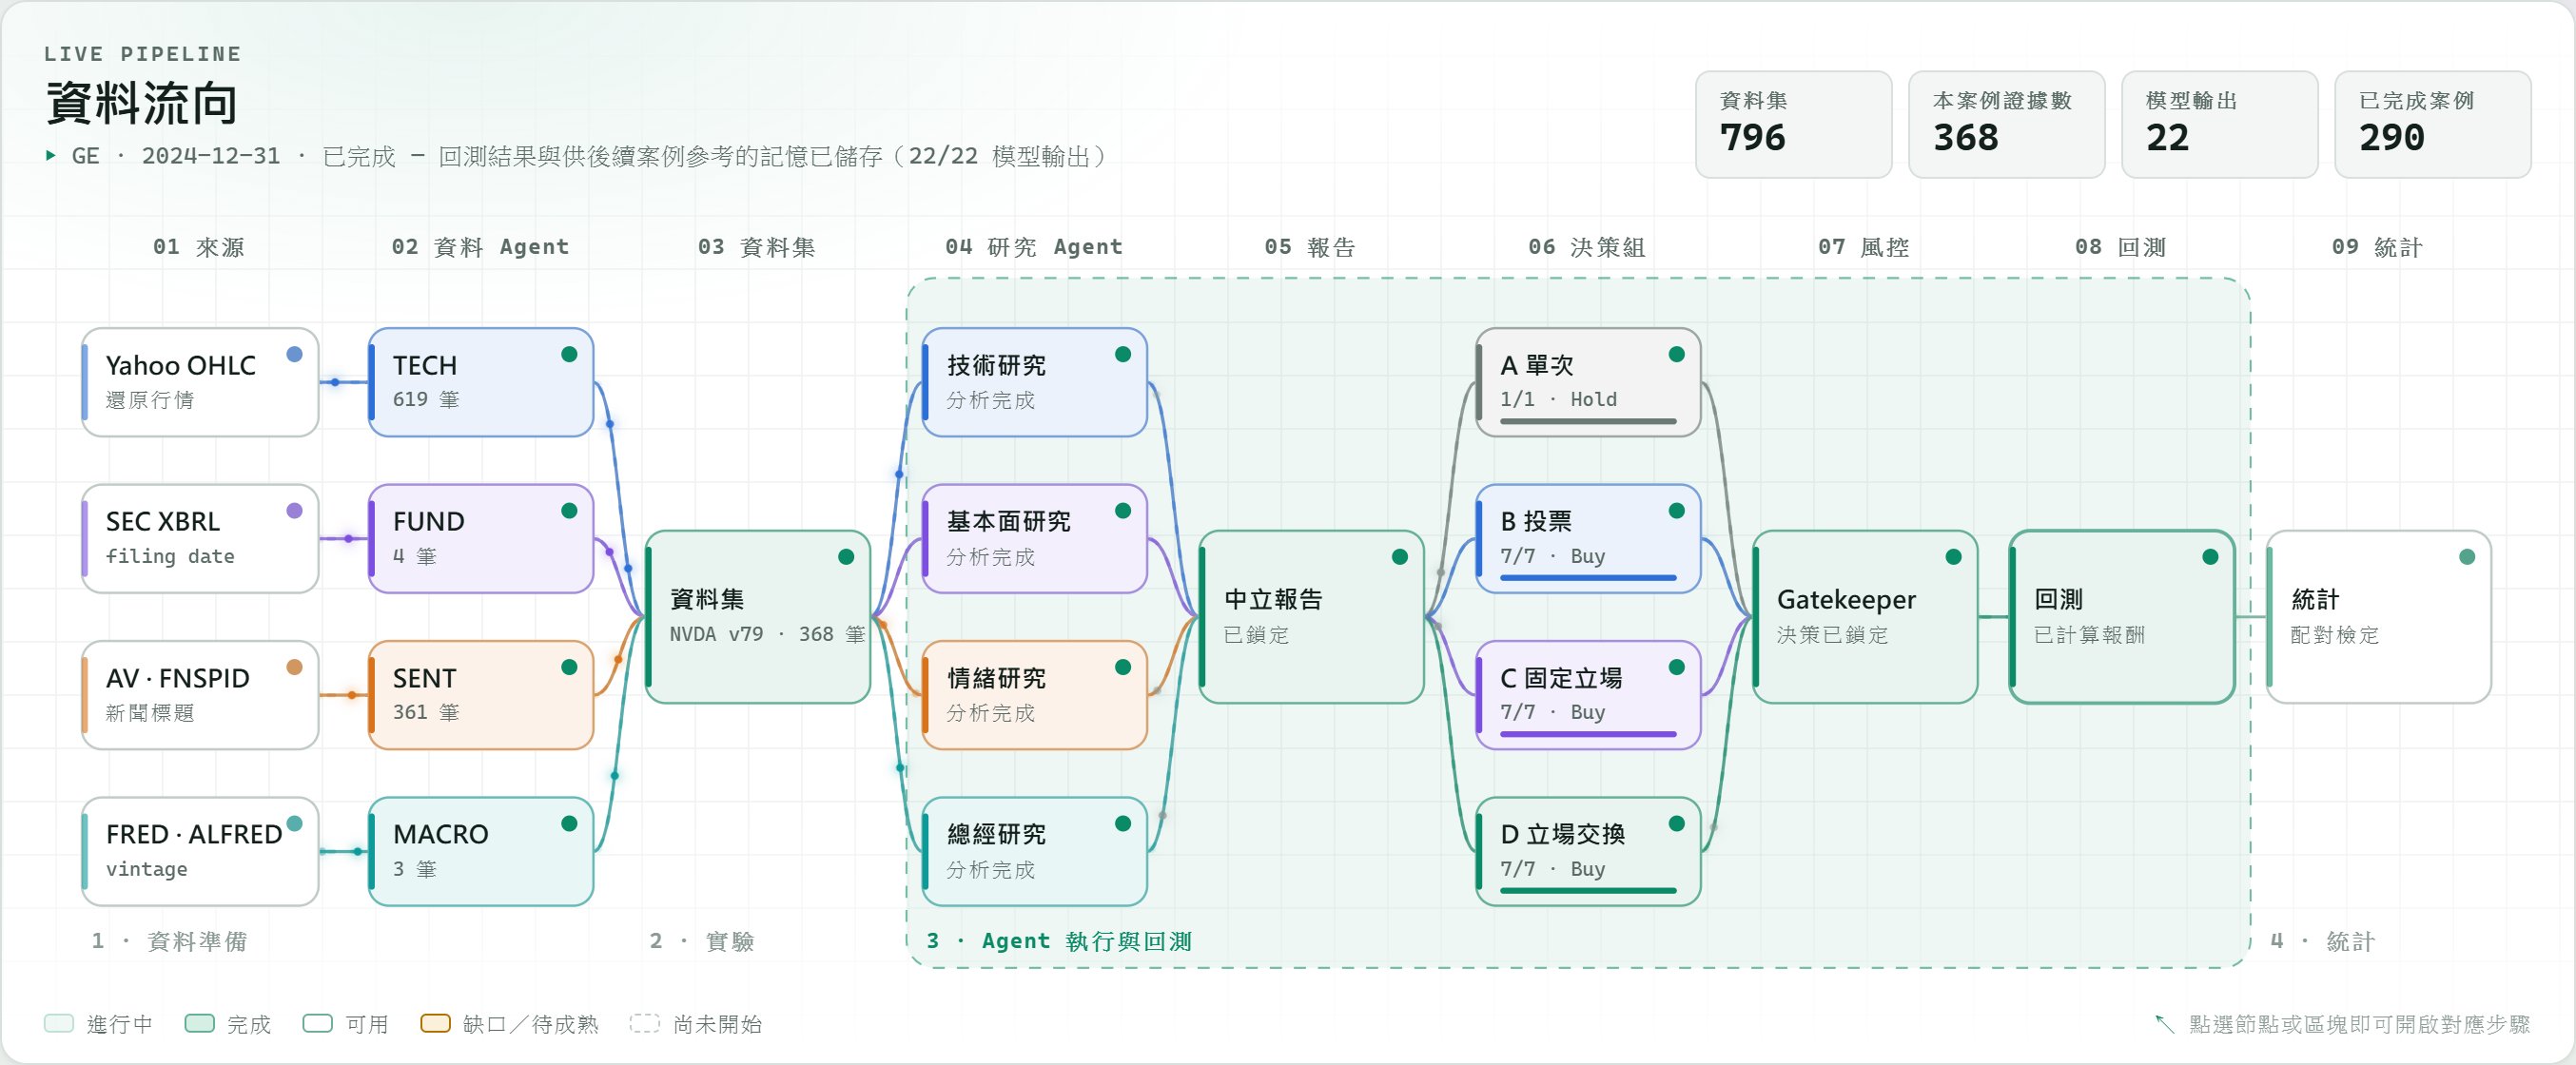
\includegraphics[width=\textwidth]{figures/ui-pipeline.png}
\caption{網頁介面的資料流向圖（一個已完成的案例）。由左至右依序為資料來源、資料代理人、資料快照、研究代理人、中立報告、四組決策、守門員、回測與統計。}
\label{fig:ui}
\end{figure}


介面以執行狀態與來源追蹤來支援研究檢查；模型的指派、論證、裁決與資源使用的紀錄，都應該能對應到單一案例。

\subsection{實作流程與驗證}

\subsubsection{開發流程}
系統依「資料、研究、決策、回測、統計」的順序逐步開發。每完成一個模組，先用模擬資料與小樣本測試，再用少量真實案例試跑，最後才進行正式實驗。開發過程中主要的挑戰與對策如下：

\begin{itemize}
  \item 時間邊界：財報與新聞要依「何時才看得到」篩選，避免分析日之後的資訊混進輸入；總經資料改用歷史版本，排除事後修正的影響。
  \item 模型輸出不穩定：模型常引用不存在的證據或輸出格式錯誤，所以用結構化輸出、證據短代稱與自動重試處理；模型也常自己改寫數字，所以改成要求用證據代稱來指稱事實。
  \item 結果可重現：系統設計上，在事前登記時鎖定程式與模型版本，每一步推理前後都核對模型權重，版本不符就拒絕執行。實際執行中仍有未完整保存的項目（FinBERT 版本、Gemini 呼叫設定、行情調整版本），見\frref{sec:repro}。
  \item 長時間執行：網路中斷時自動暫停，恢復後接著跑，已完成的步驟不重做，目的是讓 180 個案例在一致的條件下完成；180 案的原始輸出與版本對應，仍須在定稿前補齊。
\end{itemize}
\subsubsection{稽核紀錄與版本核對}
系統設計要求模型輸出在寫入前先驗證，並為每次呼叫建立稽核紀錄。下列項目是系統所支援的紀錄內容；現有 180 案是否全部具備完整紀錄，仍須以最終匯出清單逐案核對：

\begin{itemize}
  \item 提示詞中的證據用短代稱（E1、E2、$\ldots$）呈現，模型回答後再由程式對應回真正的識別碼。這樣可以避免模型抄錯很長的識別碼，也避免識別碼裡的申報編號洩漏公司身分。
  \item 引用的證據必須存在；如果引用不存在的證據或格式錯誤，系統會用明確的訊息要求重試，最多三次。
  \item 數字檢查：新版要求代理人用證據代稱指稱事實，而不是重述數字。敘述中如果還是出現沒有任何證據數值支持的數字（期間名稱、日期、來源值的四捨五入或截位不算），只記錄下來並依組別報告比例，不重試，也不修改文字。
  \item 凍結與身分核對：每一步推理前後，都核對模型權重的指紋碼；取不到時就暫停，之後可以接續執行；如果確認前後不同，該案例就永久作廢。程式原始碼的雜湊值也納入實驗規則的雜湊值，只要程式被改動就拒絕續跑。連線故障連續發生時，會暫停派發新案例，停滯太久時自動關閉 GPU 主機。
  \item 系統支援逐案匯出實驗規則設定、中立報告、證據登錄、執行軌跡、記憶、決策、逐案例回測、彙總指標與辯論逐字稿；本文不以此功能宣稱現有 180 案已全部完成可重現性核對。
\end{itemize}
\subsection{實作上的挑戰}

\subsubsection{格式不同與輸入長度限制}
不同模型的結構化輸出格式、分詞方式（tokenizer）與可讀的內容長度各不相同。轉接程式不能偷偷加入額外的金融資訊，也不能默默截掉某一方的反面證據。所以需要統一輸出格式、保存模型的原始回應與截斷紀錄，限制輸入長度並記錄失敗的情況。

\subsubsection{資源公平與領域輸出標準化}
呼叫次數相同，不代表 token 用量、成本或延遲相同；四個領域平行執行時，實際花費的時間與累計的推理時間也會不一樣。各領域看法的長度、缺漏值、證據與反面證據欄位如何標準化，會影響上層的裁決，因此格式與提示詞必須先鎖定，不能看完績效再調整權重。

\subsubsection{模型能力造成的混淆}
有了模型路由，並不表示就能識別出「異質性」本身的效果。模型能力的組合、裁決者對某種文風的偏好，以及不同模型的訓練記憶風險，都可能影響比較結果，所以要靠分開設定模型條件、控制輸入內容，並限定結果的適用範圍來解讀。

\clearpage\section{結果與討論}
\subsection{既有實驗規則下的機制比較}
本節呈現 qwen3:32b、季度實驗規則 v3-1002.3 下的既有回溯比較，以及同一批案例的 Gemini 探索性分析。結果只適用於這個模型、這套流程與這批資料；本節不能當成「不同模型辯論」或「領域專業化架構」的績效證據。


\subsubsection{qwen3:32b 的績效與配對檢定}
180 個案例（季度實驗規則 v3-1002.3）全部完成，沒有排除任何案例。表~\ref{tab:main} 是四組的績效，表~\ref{tab:tests} 是配對檢定。

\begin{table}[H]
\centering\small
\caption{四組績效（180 案，60 個交易日，已扣除交易成本）}
\label{tab:main}
\setlength{\tabcolsep}{5pt}
\begin{tabular}{@{}lccccc@{}}
\toprule
組別 & 出手率 & 條件準確率 & 累積報酬 & 最大回撤 & 年化 Sharpe \\
\midrule
\grp{A}\ 單次判斷 & 78.3\% & 56.0\% & 1.85\% & $-1.81\%$ & 0.44 \\
\grp{B}\ 獨立投票 & 79.4\% & 55.9\% & 1.95\% & $-1.83\%$ & 0.46 \\
\grp{C}\ 固定立場辯論 & 100\% & 58.3\% & 2.51\% & $-1.47\%$ & 0.59 \\
\grp{D}\ 立場交換辯論 & 100\% & 55.0\% & 2.11\% & $-2.01\%$ & 0.54 \\
\midrule
買進持有（同案同期間） & -- & -- & 5.60\% & $-1.59\%$ & 1.01 \\
\bottomrule
\end{tabular}
\par\smallskip
\raggedright\footnotesize 決策是守門員處理之前的候選決策。「出手率」是決定買進或賣出（不是持有）的案例比例；方向準確率只用有出手的案例計算。這裡把每個「股票×分析日」案例視為一個固定權重（1/180）的部位，只在該案例 60 日持有期間依決策做多或放空，其餘時間、以及決定持有的案例，都以零報酬的現金計算，所以不同案例的持有期間可能重疊。買進持有的基準採相同的配置：在每個案例的相同期間做多該股票，不是九檔股票全期間一直持有。
\end{table}

\begin{table}[H]
\centering\small
\caption{立場交換辯論（\grp{D}）的配對檢定（60 個交易日）}
\label{tab:tests}
\setlength{\tabcolsep}{4pt}
\begin{tabular}{@{}lcccccc@{}}
\toprule
比較 & 配對案例 & 方向不同 & 準確率差 & McNemar $p$ & Sharpe 差 & Ledoit--Wolf $p$ \\
\midrule
\grp{D} 對 \grp{C}（主要） & 180 & 16 & $-3.3$ & 0.21 & $-0.05$ & 0.80 \\
\grp{D} 對 \grp{B} & 143 & 9 & $+0.7$ & 1.00 & $+0.08$ & 0.79 \\
\grp{D} 對 \grp{A} & 141 & 8 & $+1.4$ & 0.73 & $+0.10$ & 0.72 \\
\bottomrule
\end{tabular}
\par\smallskip
\raggedright\footnotesize 準確率差的單位是百分點。主要比較經 Holm 校正後的 $p$ 值為 0.42（準確率）與 0.80（Sharpe）。與 \grp{A}、\grp{B} 比較時，方向準確率與 McNemar 檢定只限兩組都有出手的配對案例；Sharpe 差與 Ledoit--Wolf 檢定，則使用各組在共同交易日上的完整組合日報酬序列，持有及非交易期間依既定規則記為零。配對案例數並不等於 Sharpe 檢定所用的日序列筆數。
\end{table}

在主要比較中，\grp{D} 的方向準確率與 Sharpe 比率都略低於 \grp{C}，但差異並不顯著。以日期分組計算，準確率差的 95\% 信賴區間是 $[-7.2, +0.6]$ 個百分點，Sharpe 差的區間是 $[-0.47,+0.36]$。30 與 90 日、不計成本、守門員之後的決策、排除 37 個新聞來源／覆蓋診斷案例等敏感性分析，都沒有提供 \grp{D} 優於 \grp{C} 的顯著證據；但有些點估計的方向不同（例如 30 日的 Sharpe 差是 $+0.04$）。四組的 Sharpe 點估計都低於相同配置的買進持有參照（我們沒有對這個基準做優越性檢定）。

\paragraph{與研究目的對照。} 研究問題是「自我反駁式立場交換，是否優於固定立場辯論」。依事前指定的判定標準，兩個主要指標都沒有顯著為正，所以不支持立場交換優於一般辯論。兩個辯論組的 Sharpe 雖然高於 \grp{A}、\grp{B}，但辯論組必須出手（不能選持有），在以上漲為主的期間，持有的時間較少，因此這個差異不能歸因於辯論本身。

\paragraph{與簡單基準的比較。} 在 180 案全部納入的條件下，\grp{C}、\grp{D} 的準確率（58.3\%、55.0\%）點估計都低於「一律看多」的 62.2\%（表~\ref{tab:flash}，說明見\frref{sec:gemini}）。「一律看多」與 C、D 只在 C、D 決定賣出的案例上不同，所以可由表~\ref{tab:confusion} 做配對的精確 McNemar 檢定（事後、探索性，未對多重比較校正）：C 賣出的 35 案中，C 對而一律看多錯的有 14 案，反過來有 21 案（$p=0.31$）；D 賣出的 43 案中，分別是 15 案與 28 案（$p=0.07$）。兩者都沒有達到 0.05，但點估計都不利於辯論組。Sharpe 相對買進持有的比較需要完整的日報酬序列，目前尚未檢定。因此，這批資料沒有顯示任何一種辯論流程勝過最簡單的基準；所以即使 \grp{D} 與 \grp{C} 有差異，也不能由此推論辯論流程本身具有可用的預測力。

\paragraph{檢定力與「算作一樣好」的界線。} 研究事前沒有訂下「兩組算作一樣好」或「不比較差」的界線，所以不能因為結果不顯著，就說兩組相同或不比較差。若固定觀察到的 16 個方向不一致的案例，並暫時假設各案例互相獨立，對單一的準確率指標做雙尾 $\alpha=0.05$ 的精確檢定，要有 80\% 的機會偵測到差異，預期差距約需 6.3 個百分點（這稱為「最小可偵測差距」）。這個數字沒有考慮日期之間的相依，也沒有考慮 Holm 校正與 Sharpe 的聯合門檻，更不是事前做的檢定力規劃。

\paragraph{決策分布。} 180 案中，有 129 案（72\%）四組的決策完全一樣，\grp{C} 與 \grp{D} 只有 16 案方向不同。以候選決策來看，四組都以買進為主（\grp{A} 買進 108、持有 39、賣出 33 案；\grp{B} 109、37、34 案；\grp{C} 買進 145、賣出 35 案；\grp{D} 買進 137、賣出 43 案），\grp{D} 的賣出比 \grp{C} 多。守門員只對 INTC 2024-09-30 這一案出手：因為波動度過高，把四組的賣出都降為持有。\grp{A} 與 \grp{B} 的買進、持有與賣出總數接近，只代表整體分布相似；逐案是否一致，還要等原始決策匯出後才能核對，所以我們不據此推論「七次投票」與「單次判斷」是等價的。
\subsubsection{正反分歧的案例與可能的解釋}

以下案例是在結果揭曉之後才挑選的，只用來描述，不能用來判斷因果機制。這裡的判定標準適用於季度實驗規則 v3-1002.3；少數案例也不能代表全部 16 個方向不同的案例。
\paragraph{案例一：INTC 2024-03-31（\grp{D} 正確）。} 研究報告顯示新聞情緒偏正面、近 20 日報酬為正，但營收、淨利與營業現金流都比去年同期大幅衰退。表~\ref{tab:case} 是兩組的辯論與裁決摘要（代理人原文是英文，這裡是摘要翻譯）。

\begin{table}[H]
\centering\small
\caption{案例一：INTC 2024-03-31 的辯論與裁決（60 日實際報酬 $-30.5\%$）}
\label{tab:case}
\begin{tabularx}{\textwidth}{@{}L{.17} L{.22} Y@{}}
\toprule
組別／輪次 & 立場與預測 & 論點摘要 \\
\midrule
\grp{C} 第 1--3 輪 & 第 1 輪：看多 $+8\%$；看空 $-12\%$ & 看多方三輪幾乎都在重複「情緒正面與短期動能支持看多」；看空方也一直重複財報衰退，雙方都沒有回應對方的核心證據（各輪預測值逐輪的變化，須由原始輸出核對） \\
\grp{C} 裁決 & 買進，$+5\%$ & 採納看多方的短期動能論點 \\
\midrule
\grp{D} 第 1 輪 & 看多 $+8\%$；看空 $-10\%$ & 論點方向與 \grp{C} 相同（預測值略有差異） \\
\grp{D} 第 2 輪 & 原本看多的一方改看空，$-7\%$ & 引用並反駁自己原本的主張：正面情緒與短期報酬「被營收、淨利與現金流的大幅衰退所抵銷」 \\
\grp{D} 裁決 & 賣出，$-7\%$ & 基本面惡化的重要性高於短期情緒 \\
\bottomrule
\end{tabularx}
\end{table}

這個案例中可以看到，交換輪特別強調了原本被輕描淡寫的基本面衰退，最後裁決也轉為賣出；60 日後股價下跌 30.5\%，\grp{C} 判斷錯誤，\grp{D} 判斷正確。由於本段只分析主要的 C／D 比較，未經原始輸出逐案核對的 A／B 決策不在此列示。

\paragraph{案例二：AAPL 2023-03-31（\grp{D} 錯誤）。} 這個案例的技術面很強（近 20 日上漲 11.3\%），但營收與淨利比去年下降。\grp{C} 採納技術動能的判斷，決定買進；\grp{D} 的交換輪則再次強調基本面衰退，裁決者因此判斷賣出。60 日後股價上漲 15.3\%，\grp{D} 錯了。

\paragraph{整體模式。} 在 16 個方向不同的案例中，\grp{D} 有 12 案判斷賣出；就這 16 案整體而言，D 對 5 案、C 對 11 案。兩個案例都看得到，交換輪會強調反面證據（多半是基本面衰退），而且 \grp{D} 的最終決策比較常轉為看空，這與自我反駁的設計目的相符；但案例太少，不足以確定其中的因果。一個可能的解釋是：本研究的期間以上漲為主，「基本面疲弱但股價還是繼續漲」的情形比較多，所以比較常看空反而吃虧。此解釋的事後檢驗見\frref{sec:gemini}的「事後檢驗：\grp{D} 偏空的解釋」。兩組的部分文字與決策確實不同，但這並沒有顯示 D 比較好；也不能把差異全部歸因於交換立場。這個結論與「辯論效果常被高估」的文獻一致 \citep{smit2023mad,zhang2025stop}。
\subsection{探索性的跨模型分析與前導診斷}

\subsubsection{Gemini 同一模型的比較}
\frlabel{sec:gemini}

把整套系統改用 Gemini，仍然是單一模型的設定，和 RQ2 要研究的「同一場辯論裡使用不同模型」不同。以下呈現同一批案例的探索性模型替換比較，以及解讀時的界線。


以下分析都是在主要結果揭曉之後才做的，沒有事先登記。依照 \citet{wagenmakers2012agenda} 與 \citet{nosek2018prereg} 的區分，這屬於探索性分析，只能用來產生後續研究的假說，不能當作確認性的證據。

\paragraph{跨模型比較。} 我們用 Gemini 3 Flash，依照相同的案例集合、流程與匿名化設定，把四組重新跑一遍（表~\ref{tab:flash}）。結果與 qwen3:32b 一致：\grp{D} 的準確率仍略低於 \grp{C}；\grp{C}、\grp{D} 方向不同的案例只有 9 案（\grp{D} 單獨正確 3 案、\grp{C} 單獨正確 6 案，McNemar $p=0.51$）。這是在相同標的、日期與來源資訊上換模型的比較，不是用獨立資料重做一次。現有匯出的紀錄，不足以證明兩個模型的完整呼叫設定與逐案的研究報告完全一致，所以不能說兩個模型一字不差地讀到同一份報告，也不能把換模型的結果當成單純的「能力改變」。兩個模型的決策高度相似，\grp{C}、\grp{D} 分別有 165 與 162 案的方向相同。

\begin{table}[H]
\centering\small
\caption{跨模型比較：方向準確率（60 日、候選決策、有出手的案例）}
\label{tab:flash}
\begin{tabular}{@{}lcc@{}}
\toprule
組別 & qwen3:32b & Gemini 3 Flash \\
\midrule
\grp{A} 單次判斷 & 56.0\% & 57.6\% \\
\grp{B} 獨立投票 & 55.9\% & 56.7\% \\
\grp{C} 固定立場辯論 & 58.3\% & 57.8\% \\
\grp{D} 立場交換辯論 & 55.0\% & 56.1\% \\
\midrule
一律看多（全部 180 案；只能與 C／D 比較） & \multicolumn{2}{c}{62.2\%} \\
\bottomrule
\end{tabular}
\par\smallskip
\raggedright\footnotesize 兩個模型都報告 180 案。qwen 的 A、B 有出手的案例分別是 141、143 案（覆蓋率 78.3\%、79.4\%），C、D 是 180 案。現有的 Gemini 彙總資料沒有提供可以核對的 A／B 出手數與覆蓋率；C、D 依強制下注規則為 180 案。A、B 的條件準確率只涵蓋有出手的子集，不能直接與全樣本的 62.2\% 比較。
\end{table}

\paragraph{與「一律看多」的比較。} 180 案中有 112 案在 60 日內上漲（62.2\%）、68 案下跌（37.8\%）。只有涵蓋全部案例的 \grp{C}、\grp{D} 可以直接與這個「事後才知道的方向」比較；兩個模型的這兩組準確率，點估計都比它低。對 qwen 而言，表~\ref{tab:confusion} 是由既有的決策總數與正確數重建出完整分布，不是新的逐案驗證。賣出的精確率（賣出的案例中，真的下跌的比例）分別是 40.0\%（14/35）與 34.9\%（15/43），和全樣本的下跌率 37.8\% 相比，一個較高、一個較低；下跌的召回率（所有下跌案例中，被猜到要賣出的比例）分別是 20.6\% 與 22.1\%。所以，只能說這兩組對下跌的召回偏低，不能概括說它們完全沒有辨識力。

\begin{table}[H]
\centering\small
\caption{qwen3:32b 的方向混淆分布（60 日，候選決策）}
\label{tab:confusion}
\begin{tabular}{@{}llrrr@{}}
\toprule
組別 & 預測方向 & 實際上漲 & 實際下跌 & 合計 \\
\midrule
\grp{C} & 買進 & 91 & 54 & 145 \\
         & 賣出 & 21 & 14 & 35 \\
\grp{D} & 買進 & 84 & 53 & 137 \\
         & 賣出 & 28 & 15 & 43 \\
\bottomrule
\end{tabular}
\par\smallskip
\raggedright\footnotesize 每組總數為 180；正確數 C=105、D=99。這是由既有彙總數用代數重建的，不當作額外的逐案驗證。A／B 的持有分布與 Gemini 的完整分布，也不從四捨五入後的準確率反推。
\end{table}

\paragraph{事後檢驗：\grp{D} 偏空的解釋。} 本研究原本推測：\grp{D} 比較常看空，所以在多頭時期吃虧，在空頭時期應該會比較好。我們把 20 個分析日，依九檔股票的平均 60 日報酬分成 6 個空頭季與 14 個多頭季，結果 \grp{D} 在空頭季的準確率也沒有高於 \grp{C}（qwen 是 24.1\% 對 25.9\%；Flash 是 25.9\% 對 27.8\%），兩個模型都只差一個案例，而且季別是事後才分類的。所以這份資料沒有支持上述推測，但也不能說已經推翻它。

\paragraph{兩個模型差異方向的描述。} 兩個模型的 \grp{D}$-$\grp{C} 準確率差都是負的，方向一致（這只是描述）；我們沒有檢定「模型與機制之間的交互作用」、「兩者是否等效」，也沒有做跨模型 Sharpe 的聯合判準。由於用的是同一批樣本、分析屬於探索性，而且模型紀錄不夠完整，所以不能說已經確認了跨模型的穩健性。

\paragraph{後續假說。} 在兩個模型的既有準確率結果中，我們都沒有看到 \grp{D} 帶來改善。輸入資訊本身的預測力不足，是可能的解釋之一，但市場雜訊與效率、提示詞設計、模型限制、樣本數與生成的隨機變動，也都可能造成這個結果；本文沒有用實驗把這些原因分開。後續可以用新的期間或新的標的，先登記好擴充資訊與消融（逐項拿掉看影響）的方案，再檢驗跨標的的訊號是否真的有額外價值 \citep{nosek2018prereg}；不能在產生假說的同一批資料上，把探索結果改稱是確認性的證據。
\subsubsection{記憶與匿名辨識探針}
\frlabel{sec:memorydiagnostic}

專案已保存 2026 年 9 月 28 日 qwen3:32b 的前導探針。其中「無資料回想」測試用了 63 題、60 日期間、溫度 0、種子 905：2022、2023、2024 年各 9 題，方向正確率分別是 33.3\%、33.3\%、55.6\%，2025 年 36 題為 72.2\%，都沒有高於各組的「多數方向基準」（66.7\%、66.7\%、55.6\%、72.2\%）。這只能說，用這種問法沒有看到「超出基準的回想表現」，並不能證明模型沒有記憶。

另外，我們拿 2023-06-30 與 2024-06-30 各九檔股票的匿名證據前 6,000 字元，詢問「這是哪家公司」，qwen 辨識出 6/18（33.3\%）；產品名稱與財報規模仍然提供了線索。這是開放式的回答，不是九選一的測試，所以不直接用 1/9 當作統計上的「純猜」基準。這兩項探針使用的是前導階段的實驗規則 39f71a9c，沒有完整保留可以比對的模型權重與新版研究報告的身分，所以不能當作 v3-1002.3 全部 180 案的辨識率。專案另有 Gemini 2.5 Flash 等其他模型的探針，也不能取代對本批 Gemini 3 Flash 的汙染檢驗。


\subsection{研究限制}

\subsubsection{資料有效性}
九檔股票是以「資料取得容易」為主挑選的，沒有納入已下市的公司，所以有存活偏誤與事後選樣的風險。財報申報日、總經歷史版本與新聞時間戳記，控制了資料「何時可得」，但無法排除模型訓練時的記憶；匿名化之後仍保留數值、日期與產品線索。行情用的是下載當時的調整版本，也有事後被修訂的風險。新聞來源與數量會隨年份與個股而改變；排除 37 案的分析只是來源與覆蓋範圍的診斷，不能推廣成統一的新聞數量門檻。

\subsubsection{實驗有效性}
D 同時包含立場交換、隔離對手、強制引用與驗證重試，所以估計的是整套流程的差異，不是單獨立場交換的效果。預定呼叫次數相同，不代表重試次數、token 或運算量也相同。C、D 必須下注、而且可以用已到期的記憶；A、B 可以選持有、也沒有記憶，所以補充比較混合了好幾項差異。每個案例只生成一次，所以觀察到的 C、D 分歧，也可能包含生成時的隨機雜訊。同一批資料已經用於前導試跑與規則調整，規則鎖定之後，也無法恢復「未見過樣本」所應有的確認性。

不同模型的能力組成與訓練記憶差異，很難完全分開；溫度或種子設成一樣，也不代表生成機制相同。領域切分可能遺失跨領域的互動，上層整合也會受到輸入順序、長度與文風影響。模型輸出的多樣性或論述的豐富程度，不能直接當成績效改善的證據。

\subsubsection{統計有效性}
180 個案例共用 20 個分析日，持有期間也有重疊，而主要的 C／D 比較只有 16 個方向不一致的案例。依日期分組的信賴區間，只用來檢查相依性造成的影響，不能當成「一樣好」或「不比較差」的證據；最小可偵測差距也不是事前的檢定力規劃。因為事先沒有訂定「算作一樣好」的界線，所以不能用不顯著的結果，宣稱兩種流程相同。Sharpe 是用對齊後的日序列計算的，其觀測數 $T$ 與案例數 180、日期分組數 20，三者不能互相替換。

\subsubsection{外部有效性與可重現性}
\frlabel{sec:repro}
結果只限於九檔美國大型股、2021--2025 年，以及指定的模型與實驗規則，不能推廣到整個市場。Gemini 的比較用的是同一批案例，不是獨立重做；現有匯出紀錄也不能支持「兩個模型一字不差地讀到相同研究報告」的說法。FinBERT 的版本、完整的 Gemini 呼叫設定與行情調整版本，紀錄不夠完整，限制了精確重現。既有小樣本匿名探針的辨識率，也不代表全部 180 案。回測中的放空部位沒有計入借券費用，也沒有逐案檢查該股票在當時是否真的能被放空；行情使用含拆股與股利調整的價格，但沒有另外模擬股息對放空部位的影響。這些設定會讓放空的報酬偏樂觀；九檔都是大型股，影響可能較小，但本文沒有量化。紀錄完整度的現況整理於表~\ref{tab:prov}；標示「部分具備」或「不完整」的項目，在補齊之前，本文的結果只能視為回溯比較，不能視為可完整重現的確認性結果。

\begin{table}[H]
\centering\small
\caption{可重現性紀錄的現況}
\label{tab:prov}
\begin{tabularx}{\textwidth}{@{}L{.25} L{.15} Y@{}}
\toprule
紀錄項目 & 現況 & 說明 \\
\midrule
事前登記時間與實驗規則雜湊值 & 已核對 & 快照登記時間為 2026-10-02 05:35:33 UTC；協議雜湊開頭為 \texttt{b1da80ee}。180 案均通過登記時間與樣本資格篩選 \\
模型身分 & 部分具備 & 登記文件載明預期的模型權重指紋碼開頭為 030ee887880f…；實際執行的指紋碼須由逐步核對紀錄確認 \\
180 案原始輸出與清單 & 已封存核對 & 180 份資料內容雜湊均符合 ID；3,960 筆決策紀錄皆有原始回應。已封存清單與 SHA-256，尚未作語意層逐句人工審核 \\
計算程式版本 & 已核對計算版本 & 使用提交 \texttt{eb36a8a} 的 reporting 原始碼；statistics、backtest、splits 與該提交相同。此為歷史程式重算，不宣稱重新啟動原容器映像 \\
配對日報酬序列 & 已保存重算 & 共 1,219 個交易日；重算 C／D Sharpe 為 0.5913／0.5384，McNemar $p=0.2101$、LW $p=0.8015$，與原表四捨五入後一致 \\
長期記憶實際內容 & 邊界已核對 & 已核對 6,804 筆記憶之同股、同組、同協議、期間、成本、守門後層與到期邊界，未發現違規；這不證明記憶對推理的語意影響 \\
FinBERT 版本、Gemini 呼叫設定、行情調整版本 & 不完整 & 限制精確重現，已於上文說明 \\
\bottomrule
\end{tabularx}
\end{table}


\clearpage\section{結論與建議}

\subsection{研究發現與對研究問題的回應}

在本報告列出的既有 180 案回溯比較中，立場交換辯論（D）的方向準確率是 55.0\%，固定立場辯論（C）是 58.3\%；年化 Sharpe 分別是 0.54 與 0.59。D 相對於 C 的兩項差異，都沒有達到事先訂定的「優越」判準，因此目前的資料不支持「整套 D 流程優於整套 C 流程」。這並不代表兩組一樣好；而且 D 同時包含立場交換、隔離對手、強制引用與驗證重試，也不能把結果歸因於單一的「立場交換」因素。

另一項值得注意的結果是：C、D 的準確率（58.3\%、55.0\%）點估計都低於「一律看多」的 62.2\%，四組的 Sharpe 也都低於同配置買進持有的 1.01。準確率相對「一律看多」的事後配對檢定也未顯著（C 的 $p=0.31$，D 的 $p=0.07$），Sharpe 相對買進持有則尚未檢定；本樣本的點估計未超過上述簡單基準，但這不構成統計劣勢或一般性無效的證據。案例觀察只是描述，不能用來判斷因果機制。

RQ2 的模型組合與 RQ3 的領域決策分工，仍然是後續設計，目前沒有任何實驗結果；它們檢驗的是兩個候選假說，並非已被證實的原因。既有結果的原始輸出與版本對應仍未全部補齊。因此，本專題目前可支持的貢獻，是呈現一個受限條件下的 C／D 回溯比較、如實報告未觀察到優越性的結果，並整理後續可檢驗的研究設計；尚不能宣稱已建立一般化的投資方法或完全可重現的評估框架。

\paragraph{2026 年 10 月 15 日重算補記。} 從本機保存的 RQ1 快照透過 SQLite backup 建立隔離副本，以唯讀方式驗證 180 個登記案例與資料內容，再以歷史計算程式重算。兩端點 Holm 校正後的 $p$ 值為 0.420227 與 0.8015，既有負面結果不變。證據包包含逐案資料、原始輸出、記憶、日面板、計算原始碼與完整性清單；來源副本的 SHA-256 在重算前後一致。此補件提高結果的可查核性，但不使已見過的樣本成為新的確認性樣本。

\subsection{應用與價值}

\subsubsection{可追溯的決策輔助}
在應用上，本系統是一個投資研究流程原型：它把資料整理、正反論證、裁決理由與回測結果放在同一流程中，目標是讓使用者能追查建議依據，而不是只得到買賣訊號。由於現有紀錄仍有缺漏，而且績效沒有勝過簡單基準，本文不宣稱它已是有效的投資決策工具。在方法上，本研究透過預定呼叫次數對齊、規則登記、匿名化、版本鎖定與稽核紀錄，嘗試提高語言模型代理人比較的可追溯性。不過，同一批資料曾用於前導試跑與規則調整，所以規則登記不能讓它變成「未見過樣本」的確認性驗證；預定呼叫次數相同，也不能排除實際運算量的差異。這套架構目前適合作為後續多代理人受控比較的研究原型。
\subsubsection{多代理人系統設計}

研究的價值也在於：讓不同的系統設計可以被清楚地比較。只是給代理人取不同的名字，不足以證明它們有用的差異；到底需不需要不同的模型、複雜的資訊適不適合交給專才處理、領域拆分有沒有好處，都應該用受控的結果與成本來回答。如果最後沒有觀察到改善，這項研究仍然能提供「架構適用範圍」與「可重現的評估經驗」，但不能把負面結果改寫成「分工一定有用」。

\subsection{未來展望}

\subsubsection{不同時間尺度的穩健性}

未來可以比較「每季／60 日」與「每月／20 日」兩種設定，檢驗結果在不同時間尺度下穩不穩，以及較短的尺度會不會減輕資訊整合的負擔。時間尺度的改變與領域分工是兩個不同的研究因素；每月／20 日的比較會另外獨立設計，不併入本研究的 180 個季度案例。

\subsubsection{模型、路由、消融與獨立樣本外檢驗}

後續可以考慮更多模型、不同模型的裁決者、動態路由、動態辯論、領域加權、運算效率，以及不同的辯論輪數。其他延伸還包括：只讀自己、但不換立場的消融（拿掉「換立場」這一項，看效果是否還在）、空頭與高波動時期的檢查、同一案例多個種子的 C／C' 重跑，以及完整的汙染探針。需要學習參數或權重時，必須另外準備開發與驗證用的資料；最後要用新的期間或新的標的做獨立樣本外評估，不能在產生假說的同一批資料上，把探索結果改稱是確認性證據。

%% =====================================================================
%% 參考文獻（natbib + chicago；資料來自 .bib）
%% =====================================================================
\clearpage
\addcontentsline{toc}{section}{\refname}
\bibliographystyle{chicago}
\bibliography{references-meeting-20261015-v8}

\vspace{0.3cm}
\noindent\small 本文僅供學術研究與教學使用，不構成任何投資建議。
\end{document}
